\documentclass[openany,a4paper,UTF-8]{book}
\usepackage{ctex}
\usepackage{graphicx}
\usepackage{geometry}
\usepackage{color}
\usepackage{titlesec}
\usepackage{float}
\usepackage{array}
\usepackage{multirow}
\usepackage[font=small,labelfont=bf,labelsep=space]{caption}
\usepackage{titletoc}
\usepackage{titlesec}
\usepackage{fancyhdr}
\usepackage[final]{pdfpages}
\usepackage[table]{xcolor}
\usepackage{booktabs}
\usepackage{colortbl}
\usepackage{indentfirst}
%\usepackage{times}
%\usepackage{psfig}

\renewcommand{\contentsname}{Contents}

\geometry{left=3.17cm,right=3.17cm,top=2.54cm,bottom=2.54cm}
\graphicspath{{figures/}}
\setmainfont{Times New Roman}
\newcommand{\xiaoer}{\noindent\fontsize{18pt}{\baselineskip}\heiti}
\newcommand{\xiaosi}{\noindent\fontsize{12pt}{\baselineskip}\heiti}
\newcommand{\sanhao}{\noindent\fontsize{15pt}{\baselineskip}\heiti}

\newcommand{\erhao}{\noindent\fontsize{18pt}{\baselineskip}}
\newcommand{\sihao}{\noindent\fontsize{12pt}{\baselineskip}}
\newcommand{\xiaosan}{\noindent\fontsize{15pt}{\baselineskip}}

\newcommand{\song}{\fontsize{12pt}{\baselineskip}\songti}
\titleformat{\chapter}{\fontsize{18pt}{\baselineskip}\bfseries}{\thechapter}{1em}{}
\titlespacing*{\chapter} {0pt}{-12pt}{\baselineskip}
\titleformat{\section}{\fontsize{15pt}{\baselineskip}\bfseries}{\thesection}{1em}{}
%\captionsetup[figure]{labelfont={default},name={图},labelformat={default}}
\captionsetup[figure]{labelfont={default},name={Fig},labelformat={default}}

%\include{pagestyle}

\begin{document}

\thispagestyle{empty}

%\begin{titlepage}
%\begin{center}
%
\includegraphics[width=6cm]{logo}

%\Huge\textbf{ASG-GT50-C}

%\vspace{0.7cm}
%\Huge\heiti\textbf{任意序列发生器}

%\vspace{0.7cm}
%\Huge\heiti\textbf{用户手册}

%\vspace{8cm}
%\Huge\heiti\textbf{合肥量子精密仪器有限公司}
%\end{center}
%\end{titlepage}

\begin{titlepage}
\newgeometry{left=0cm,right=0cm,top=0cm,bottom=0cm}
\begin{center}
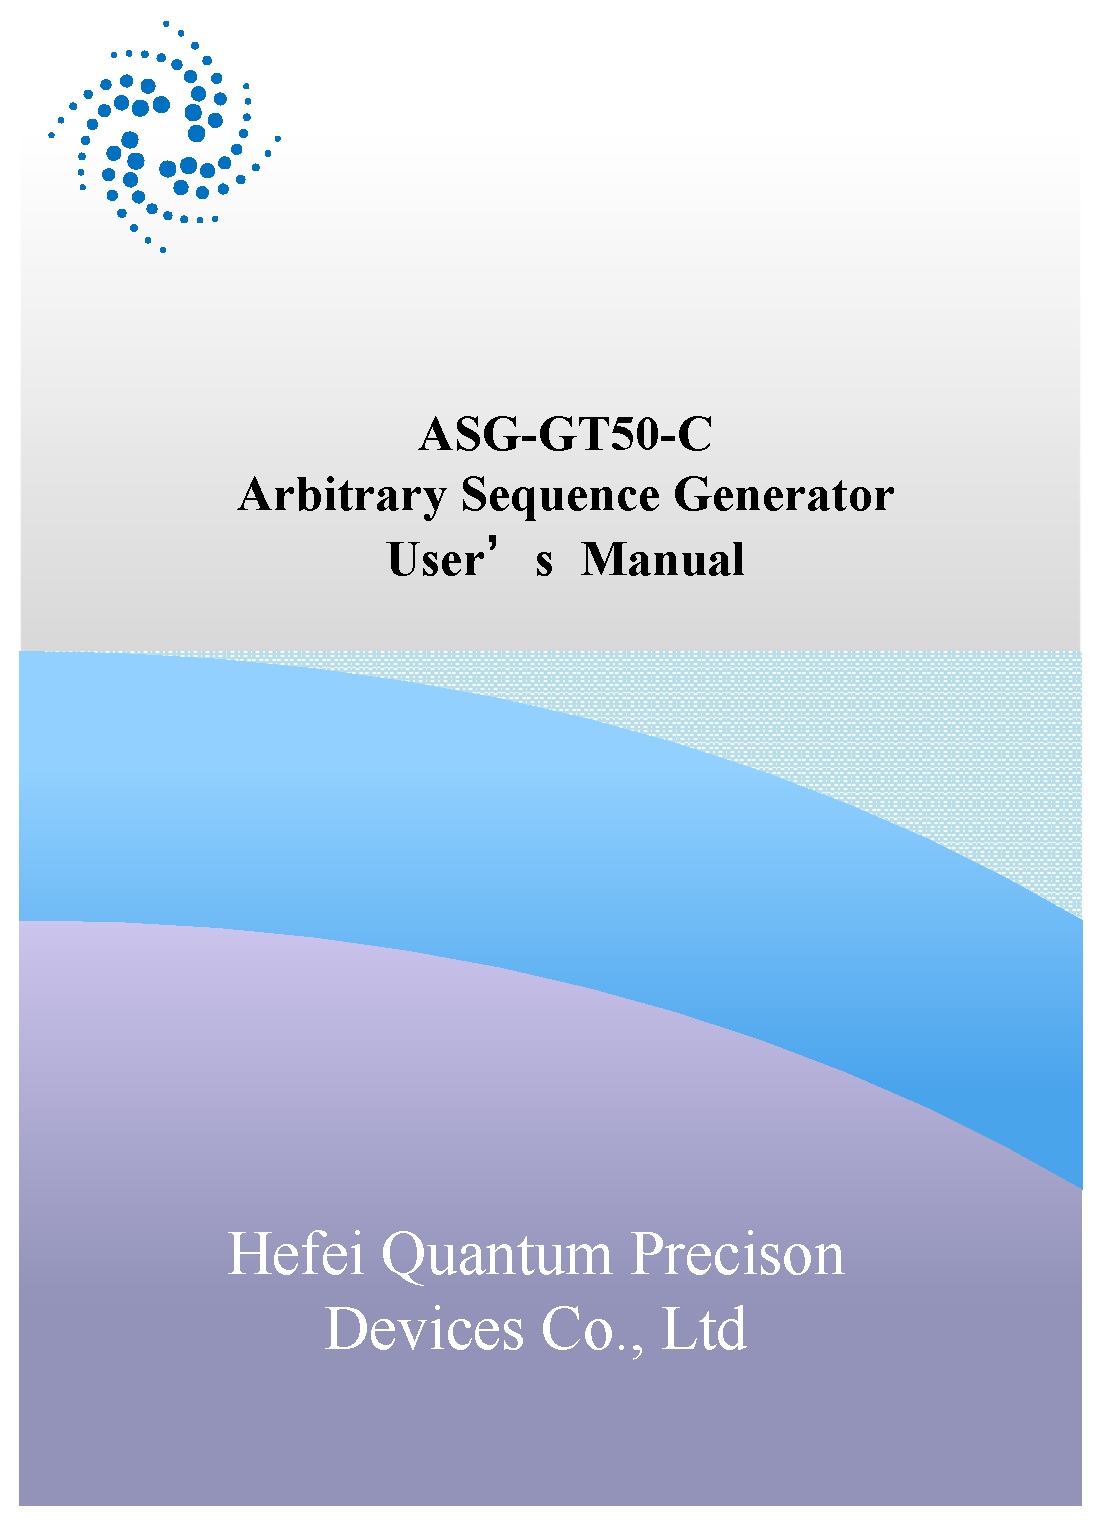
\includegraphics[width=20.99cm,height=29.69cm]{coverpage}
\end{center}
\end{titlepage}



\newpage
\qquad
\thispagestyle{empty}
\newpage
%\thispagestyle{empty}
\pagenumbering{Roman}

\newpage
%\pagestyle{empty}
\pagestyle{fancy}
\renewcommand{\headrulewidth}{2.4pt}
\renewcommand{\footrulewidth}{2.4pt}
\lhead{
    \setlength{\unitlength}{1mm}
    \begin{picture}(0,0)
    \put(0,0){
\includegraphics[width=0.9cm]{logo.eps}}
    \end{picture}
    }
\chead{}
%\rhead{\xiaosi{合肥量子精密仪器有限公司}}
%\fancyfoot[LO,RE]{\xiaosi{ASG-GT50-C用户手册}}
\rhead{\sihao\textbf{Hefei Quantum Precision Devices Co., Ltd.}}
\fancyfoot[LO,RE]{\xiaosi{ASG-GT50-C Manual}}
\cfoot{}
\fancyfoot[RO,LE]{\xiaosi\textbf{\thepage}}



\erhao \textbf{Guaranty and Declaration}
\vspace{0.7cm}

\sihao \textbf{Trademark Information}\\
%
\includegraphics[height=2cm]{logo}
%\epsfig{figure=logo,height=2cm}
%\begin{figure}[H]
%    
\includegraphics[height=2cm]{logo}
%\end{figure}
\hspace*{0.8cm}\song{\qquad\qquad is a registered trademark of Hefei Quantum Precision Devices Co., Ltd.}
\hspace{-12.2cm}
\includegraphics[height=2cm]{logo}

\vspace{0.8cm}
\sihao\textbf{Software Version}
\vspace{0.4cm}

\hspace{-0.2cm}We provide the sequence editing PC software in Windows and the interface program for both Windows (chapter 5) and MAC (chapter 6) system. Software upgrade might change or add product features. Please contact Hefei Quantum Precision Devices Co., Ltd. to upgrade the software. We will take the initiative to contact you if  necessary.
%\song 软件升级可能会增加或更改产品功能, 请联系合肥量子精密仪器有限公司升级软件, 必要时我司会主动与您联系。

\vspace{0.8cm}
\sihao\textbf{Notices}
%\song
\begin{itemize}
 \item Hefei Quantum Precision Devices Co., Ltd. products are covered by P.R.C. and foreign patents, issued and pending.
 \item Hefei Quantum Precision Devices Co., Ltd. reserves the right to change parts of or all the specifications and pricing policies at company's sole decision.
 \item Information in this publication replaces all previously corresponding material.
 \item Any part of this document is forbidden to be copied, photocopied, or rearranged without prior written approval of Hefei Quantum Precision Devices Co., Ltd.
 \item Once the users use the product, the whole content of this declaration shall be deemed to be recognized and accepted.
% \item 本公司产品受中国及其他国家和地区的专利( 包括已取得和正在申请的专利)保护。
% \item 本公司拥有改变产品规格及价格的权利。
% \item 本手册提供的信息取代以往出版的任何资料。
% \item 未经我司事先书面许可, 不得影印、 复制或改变本手册的任何部分。
% \item 用户一旦使用产品, 即视为对本声明的全部内容认可和接受。
\end{itemize}

\vspace{0.6cm}
%\xiaosi\textbf{产品认证}
%\vspace{3cm}

\sihao\textbf{Contact Us}
%\song
\begin{itemize}
 \item Xi Qin, CTO of Hefei Quantum Pricision Devices Co., Ltd.
 \item Email: sale@qpdtek.com
 \item Tel:  +86 13816630636
\end{itemize}

%\noindent\song
%如果您在使用此产品或本手册的过程中有任何问题或需求,可与我司联系:\\
%\song 秦熙: 合肥量子精密仪器有限公司, 首席技术官\\
%\song 电子邮箱: sale@qpdtek.com\\
% 电话: +86 13816630636

\newpage
\erhao \textbf{Safety Requirement}
\vspace{1.1cm}

\noindent\xiaosan\textbf{General Safety Summary}
\vspace{0.7cm}

\hspace{-0.4cm}To prevent potential hazards and avoid damage to the product or any device connected to this product, users need to understand the following safety measures, and use the instrument only specified by this manual.
%为避免可能的危险,以及防止损坏本产品和与本产品连接的任何设备,用户需了解以下安全措施,并按照规定使用本产品。

\vspace{0.7cm}
\noindent\sihao{\color{red}\textbf{Use Proper Power Cord}}

\vspace{0.2cm}
\hspace{-0.2cm}Only the power cord provided by our company should be used.
%只允许使用我司所提供的电源线。

\vspace{0.7cm}
\noindent{\color{red}\textbf{Power Supply should be Correct}}

\vspace{0.2cm}
\hspace{-0.2cm}To prevent damage to the product, please ensure the power supply is correct and read this manual carefully before using the product.
%为避免对操作人员造成伤害或损坏产品,请在使用产品前仔细阅读本手册,并确保产品供电电源正确。

\vspace{0.7cm}
\noindent{\color{red}\textbf{Do Not Operate Without Covers}}

\vspace{0.2cm}
\hspace{-0.2cm}Do not operate the product with covers removed.
%请勿在产品机箱打开时运行本产品。

\vspace{0.7cm}
\noindent{\color{red}\textbf{Avoid exposure of Circuit}}

\vspace{0.2cm}
\hspace{-0.2cm}Do not touch exposed junctions and components when the unit is powered, and please contact with us immediately.
%若机箱内电路板元件有外露, 请勿触碰并立即与我司联系。

\vspace{0.7cm}
\noindent{\color{red}\textbf{Keep Well Ventilation}}

\vspace{0.2cm}
\hspace{-0.2cm}To prevent the increase of instrument temperature which would cause damage to the product, please keep the instrument well ventilated and do not block the air vents.
%为避免因机箱内电路板过热而损坏仪器,在使用本产品的过程中请勿堵住通风口。

\vspace{0.7cm}
\noindent{\color{red}\textbf{Do Not Operate in Wet Conditions}}

\vspace{0.2cm}
\hspace{-0.2cm}In order to avoid short circuiting to the interior of the device or electric shock, please do not operate the instrument in a humid environment.
%为避免产品内部电路出现短路等危险情况, 请勿在潮湿环境下操作仪器。


\vspace{0.7cm}
\noindent{\color{red}\textbf{Do Not Operate in an Explosive Atmosphere}}

\vspace{0.2cm}
\hspace{-0.2cm}In order to avoid personal injuries or damage to the device, it is important to operate the device away from an explosive atmosphere.
%为避免人身伤害或产品损坏, 严禁易燃易爆物靠近本产品。

\vspace{0.7cm}
\noindent{\color{red}\textbf{Handling Safety}}

\vspace{0.2cm}
\hspace{-0.2cm}Please handle carefully during transportation to avoid damage to keys, interfaces, LED and other parts on the panels.
%为避免对产品面板上的按键、 接口、 指示灯等部件造成损坏, 请注意搬运安全。

\vspace{0.7cm}
\noindent{\color{red}\textbf{Do Not Place the Product in High Temperature Environment}}

\vspace{0.2cm}
\hspace{-0.2cm}To prevent potential hazards, it is forbidden to place the product in high temperature environment.
%为避免发生危险,严禁将本产品放置于高温环境中。

%\newpage
\vspace{0.7cm}
\noindent{\color{red}\textbf{People Who do not Have Ability are Forbidden to Operate the Product}}

\vspace{0.2cm}
\hspace{-0.2cm}In order to avoid personal injuries or damage to the device, people who do not have operation ability such as the olds and kids, are forbidden to use the product.
%为避免造成人身伤害或产品损坏,严禁不具备操作能力的人( 如老人、 儿童)使用本产品。

\vspace{0.7cm}
\noindent{\color{red}\textbf{General Care and Cleaning}}

\vspace{0.2cm}
\hspace{-0.2cm}Please clean the instrument regularly. To clean the exterior surface, perform the following steps: disconnect the instrument from all power sources, then clean the dust on the panel of the instrument with a dry cloth.
%请经常对产品进行清洁, 方法如下: 先断开电源, 再用干抹布轻轻擦拭产品机箱外部。

%\vspace{0.6cm}
%\noindent{\color{red}\textbf{怀疑产品出故障时, 请立即联系我司}}
%
%如果您怀疑本产品出现故障, 请联络我司授权的维修人员进行检测。 任何由未经我司允许的维护、 调整或零件更换而造成损失, 我司不承担任何责任。

\newpage
%\pagestyle{plain}
%\setcounter{page}{1}
\noindent\huge \textbf{ASG-GT50-C Series Overview}
\vspace{0.6cm}

\normalsize ASG-GT50-C serials are high performance pulse/delay generators named Arbitrary Sequence Generators. The device provides 8 independent pulse output channels. As shown in Fig 1, the width of each positive pulse could be adjusted from 7.5 ns to 2.6 s, and negative pulse could be adjusted from 10.0 ns to 2.6 s, which is no dead time with 50 ps time resolution.
\begin{figure}[ht]
\centering
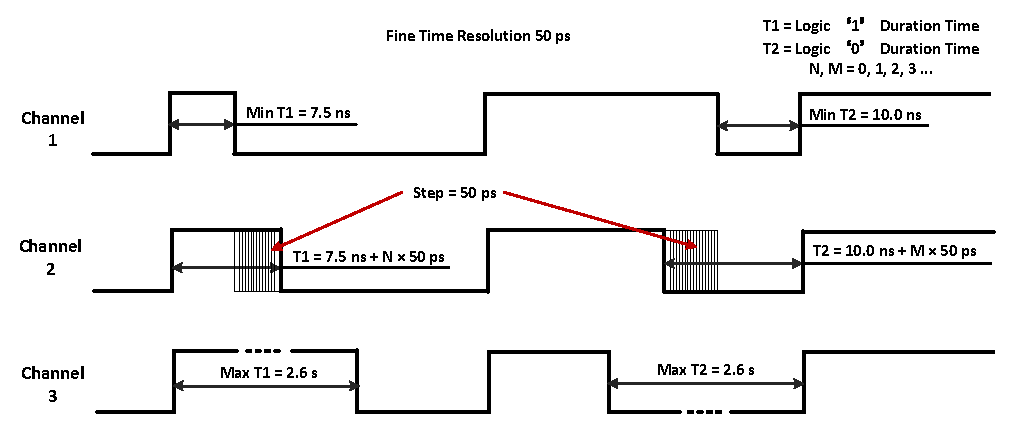
\includegraphics[width=14.5cm,height=6cm]{fig_shixu}
\caption{\hspace{0.2cm}Time diagram of pulse signals}\label{fig:fig1}
\end{figure}
\vspace{0.5cm}

\makeatletter
\def\hlinewd#1{%
  \noalign{\ifnum0=`}\fi\hrule \@height #1 \futurelet
   \reserved@a\@xhline}
\makeatother
%\newcommand\vlinewd#1{\vrule width #1}
\definecolor{myblue}{rgb}{.46,.42,.80}
\definecolor{tabcolor_top}{rgb}{255,255,255}
\definecolor{tabcolor}{rgb}{255,255,255}
\noindent\sanhao\textbf{Main Features}
%\vspace{0.1cm}
\song
\begin{table}[H]
\normalsize
\rowcolors{2}{gray!20}{gray!20}
\begin{tabular}{m{13.5cm}}
\rowcolor{gray!20}
\arrayrulecolor{tabcolor_top}\toprule[1.8pt]
Time Resolution: 50 ps\\\arrayrulecolor{tabcolor}\midrule[1.2pt]
Maximum Number of Channels: 8 \\\arrayrulecolor{tabcolor}\midrule[1.2pt]
Dynamic Range of  Single Pulse Width: from 7.5 ns  to  2.6 s\\\arrayrulecolor{tabcolor}\midrule[1.2pt]
Long-term jitter: < 25 ps (Pulse width = 500 ms) \\\arrayrulecolor{tabcolor}\midrule[1.2pt]
Sequence storage memory: 4 GB\\\arrayrulecolor{tabcolor}\midrule[1.2pt]
USB Interface\\\arrayrulecolor{tabcolor}\midrule[1.2pt]
Provide sequence editing PC software\\
\arrayrulecolor{tabcolor_top}\bottomrule[1.8pt]
\end{tabular}
\end{table}

%\begin{itemize}
% \item 50 ps时间分辨率的方波输出。
% \item 8个通道独立自定义方波输出。
% \item 单脉冲动态范围为5 ns至2.6 s,且无死时间。
% \item 高长期稳定度。
% \item 集成了高速计数读出功能。
% \item 方波序列的存储内存可以达到4 GB。
% \item 采用USB接口通信。
% \item 配备方波序列编辑软件。
%\end{itemize}

%\vspace{0.5cm}
%\newpage
\vspace{0.2cm}
%\noindent\xiaosan\textbf{Performance Characteristics}
\noindent\xiaosan\textbf{Product Specifications}
\vspace{0.5cm}

\noindent\sihao\textbf{Appearance Characteristics:}
\vspace{0.1cm}
\song
\begin{table}[H]
\normalsize
\rowcolors{2}{gray!20}{gray!20}
\begin{tabular}{m{6.5cm}|m{6.5cm}}
\rowcolor{myblue}
%\arrayrulecolor{tabcolor_top}\toprule[1.8pt]
\color{white}Parameter& \color{white}Value\\\arrayrulecolor{tabcolor}\midrule[1.2pt]
Material of the Case& Aluminium alloy\\\arrayrulecolor{tabcolor}\midrule[1.2pt]
Color& Silver gray\\\arrayrulecolor{tabcolor}\midrule[1.2pt]
Size& 207*122*65 mm\\
%\arrayrulecolor{tabcolor_top}\bottomrule[1.8pt]
\end{tabular}
\end{table}

%\begin{itemize}
 %\item 机身材质: 铝合金外壳
 %\item 机身颜色: 银灰色
 %\item 产品尺寸: 207*122*65 mm
%\end{itemize}

\vspace{0.4cm}
%\newpage
\noindent\sihao\textbf{Electrical Characteristics:}
\vspace{0.1cm}
\song
\begin{table}[H]
\normalsize
\rowcolors{2}{gray!20}{gray!20}
\begin{tabular}{m{6.5cm}|m{6.5cm}}
\rowcolor{myblue}
%\arrayrulecolor{tabcolor_top}\toprule[1.8pt]
\color{white}Parameter& \color{white}Value\\\arrayrulecolor{tabcolor}\midrule[1.2pt]
Operating Voltage& DC 12 V\\\arrayrulecolor{tabcolor}\midrule[1.2pt]
Standby Current& About 0.85 A\\\arrayrulecolor{tabcolor}\midrule[1.2pt]
Operating Current& ≤ 1.2 A\\\arrayrulecolor{tabcolor}\midrule[1.2pt]
Maximum Power& About 12 W\\
%\arrayrulecolor{tabcolor_top}\bottomrule[1.8pt]
\end{tabular}
\end{table}

%\begin{itemize}
% \item 工作电压: DC 12 V
% \item 待机电流: 约 0.85 A
%\item 工作电流: ≤1.2 A
 %\item 最大功率: 约 12 W
%\end{itemize}

\vspace{0.4cm}
\noindent\xiaosi\textbf{Technical Parameters:}
\vspace{0.1cm}
%\song
\begin{table}[H]
%\Large
\rowcolors{2}{gray!20}{gray!20}
\begin{tabular}{m{6.5cm}|m{6.5cm}}
\rowcolor{myblue}
%\arrayrulecolor{tabcolor_top}\toprule[1.8pt]
\color{white}Parameter& \color{white}Value\\\arrayrulecolor{tabcolor}\midrule[1.2pt]
Time Resolution& 50 ps\\\arrayrulecolor{tabcolor}\midrule[1.2pt]
Minimum pulse width& 7.5 ns \\\arrayrulecolor{tabcolor}\midrule[1.2pt]
Maximum pulse width& 2.6 s\\\arrayrulecolor{tabcolor}\midrule[1.2pt]
Maximum Number of Channels& 8\\\arrayrulecolor{tabcolor}\midrule[1.2pt]
Sequence storage memory& 4 GB\\\arrayrulecolor{tabcolor}\midrule[1.2pt]
Maximum Number of Pulses ( single channel )&  4×$10^{7}$\\\midrule[1.2pt]
Coupling& DC 50 ohm\\\arrayrulecolor{tabcolor}\midrule[1.2pt]
Output Low Voltage& 0 V\\\arrayrulecolor{tabcolor}\midrule[1.2pt]
Output High Voltage& 3.3 V\\\arrayrulecolor{tabcolor}\midrule[1.2pt]
%\arrayrulecolor{tabcolor_top}\bottomrule[1.8pt]
\end{tabular}
\end{table}


%\begin{itemize}
% \item  时间分辨率: 50 ps
% \item 最小脉冲宽度: 5 ns
% \item 最大脉冲宽度: 2.6 s
% \item 最大方波输出通道数: 8
% \item  方波序列存储内存: 4 GB
%\item  单通道最多输出方波个数: $4\times 10^8$个
% \item  耦合方式: DC 50 ohm
% \item  输出低电平: 0 V
% \item  输出高电平: 3.3 V
% \item  输入低电平: -5.2 V 至 +0.4 V
% \item  输入高电平: +0.6 V 至 +3.5 V
% \item  最大计数率: 50 MHz
% \item  单个计数使能信号脉冲宽度范围: 5 ns 至 5000 s
%\end{itemize}

\vspace{0.4cm}
%\newpage
\noindent\sanhao\textbf{Applications:}
\vspace{0.3cm}
\song
\begin{table}[H]
%\Large
\rowcolors{2}{gray!20}{gray!20}
\begin{tabular}{m{13.5cm}}
\rowcolor{gray!20}
\arrayrulecolor{tabcolor_top}\toprule[1.8pt]
High resolution pulse/sequence generations\\\arrayrulecolor{tabcolor}\midrule[1.2pt]
High precision synchronization \\\arrayrulecolor{tabcolor}\midrule[1.2pt]
Delay Generations\\\arrayrulecolor{tabcolor}\midrule[1.2pt]
\arrayrulecolor{tabcolor_top}\bottomrule[1.8pt]
\end{tabular}
\end{table}

\newpage
\qquad

%\begin{itemize}
 %\item 高时间精度的脉冲/序列发生器
 %\item 延时发生器
 %\item 高精度计时器
 %\item 高精度同步器
 %\item 高速计数读出
%\end{itemize}

%\newpage
\noindent\xiaoer\textbf{文档概述}
\vspace{1.3cm}

\noindent\sanhao\textbf{文档主要内容}
\vspace{0.7cm}

\noindent\xiaosi\textbf{1\quad 快速入门}
\vspace{0.4cm}

\song 介绍仪器的前面板、后面板、侧面板,以及首次使用仪器的注意事项。
\vspace{0.9cm}

\noindent\xiaosi\textbf{2\quad 仪器运行条件}
\vspace{0.4cm}

\song 介绍使用仪器所需条件,包括硬件设备条件以及运行控制软件所需条件。
\vspace{0.9cm}

\noindent\xiaosi\textbf{3\quad 软件安装}
\vspace{0.4cm}

\song 介绍仪器控制软件安装过程。
\vspace{0.9cm}

\noindent\xiaosi\textbf{4\quad 软件使用}
\vspace{0.4cm}

\song 介绍仪器控制软件的使用。
\vspace{0.9cm}

\noindent\xiaosi\textbf{5\quad 调用接口程序}
\vspace{0.4cm}

\song 介绍如何调用接口程序来控制仪器输出任意方波序列及读回计数。
\vspace{0.9cm}

\noindent\xiaosi\textbf{6\quad 故障处理}
\vspace{0.4cm}

\song 介绍在使用仪器的过程中可能出现的故障和处理方式。
\vspace{0.9cm}

\noindent\xiaosi\textbf{7\quad 注意事项}
\vspace{0.4cm}

\song 介绍在使用仪器的过程中需要注意的事项。



\newpage
\titlecontents{chapter}[0pt]{\vspace{3mm}\bf\addvspace{2pt}\filright}
              {\contentspush{\thecontentslabel\hspace{0.8em}}}
              {}{\titlerule*[8pt]{.}\contentspage}
\tableofcontents
\thispagestyle{empty}
\newpage
\thispagestyle{empty}
\qquad

\pagenumbering{arabic}
%----------------------------------------------------------------------------------------
%	CHAPTER 1
%----------------------------------------------------------------------------------------

%\chapterimage{chapter_head_2.pdf} % Chapter heading image

\chapter{Introduction}

\section{Before Starting}\index{Before Starting}

%\lipsum[1-7] % Dummy text

%------------------------------------------------

\section{Data Structure}\index{Data Structure}

%This statement requires citation \cite{book_key}; this one is more specific \cite[122]{article_key}.

%------------------------------------------------

%\section{Lists}\index{Lists}

%Lists are useful to present information in a concise and/or ordered way\footnote{Footnote example...}.

%\subsection{Numbered List}\index{Lists!Numbered List}

%\begin{enumerate}
%\item The first item
%\item The second item
%\item The third item
%\end{enumerate}
%
%\subsection{Bullet Points}\index{Lists!Bullet Points}
%
%\begin{itemize}
%\item The first item
%\item The second item
%\item The third item
%\end{itemize}
%
%\subsection{Descriptions and Definitions}\index{Lists!Descriptions and Definitions}
%
%\begin{description}
%\item[Name] Description
%\item[Word] Definition
%\item[Comment] Elaboration
%\end{description}
\chapter{\heiti Working Conditions of the Product}
\section{\heiti Hardware}
%\begin{enumerate}
%\item Windows 7或以上的操作系统的计算机一台,内存不小于1 GB。
%\item 具有USB通信接口。
%\end{enumerate}

\noindent {\textcircled{\normalsize{\textbf{1}}}}. A computer (Windows 7 or above), and the memory is greater than 1 GB.
%\noindent {\textcircled{\normalsize{\textbf{1}}}}. 计算机一台(Windows 7或以上的操作系统),内存不小于1 GB。

\noindent {\textcircled{\normalsize{\textbf{2}}}}. There is a USB interface in the computer.

\section{\heiti Software}

\noindent {\textcircled{\normalsize{\textbf{1}}}}. Python interpreter has been installed, and the version of the interpreter is  2.7

\hspace{-0.15cm}or above, but can't exceed 3.0.

%\noindent {\textcircled{\normalsize{\textbf{2}}}. Python解释器是32位的,若Python解释器为64位,我司会为您提供需要

%\hspace{-0.4em}更换的DLL文件。

\noindent {\textcircled{\normalsize{\textbf{2}}}}. Packages including wxpython, numpy, matplotlib and six have been installed.

\hspace{-0.15cm}The installation procedure will be shown in section 3.2.
%\noindent {\textcircled{\normalsize{\textbf{2}}}}. 已安装运行程序所需的各个第三方Python库,包括wxpython、numpy、

%\hspace{-0.2em}matplotlib以及six等。(安装步骤详见第3章第3.2节)

\noindent {\textcircled{\normalsize{\textbf{3}}}}. USB driver program has been installed. The installation procedure will be shown 

\hspace{-0.15cm}in section 3.3.
%\noindent {\textcircled{\normalsize{\textbf{3}}}}. 已安装USB驱动程序。(安装步骤详见第3章第3.3节)

\pagestyle{fancy}
\chapter{\heiti 软件安装}
\setmainfont{Times New Roman}

我司会为用户提供“ASG\_install”文件夹,里面包含安装仪器控制软件所需的所有文件。

\section{Python\heiti 解释器安装}
用户可到Python官网(http://www.python.org/)下载Python 2.7版本的解释器(推荐下载32位),也可直接双击运行我司提供的“ASG\_install”文件夹下“Python-2.7.11.msi”安装程序,在选择安装组件的一步时,务必勾选所有组件,然后点击“Next”即可完成安装,计算机默认会将Python解释器安装到C:\textbackslash Python27 目录下。安装完成后,打开命令提示符窗口,输入“Python” 后,如果出现如图3.1所示情况,则代表Python解释器安装成功。若得到“Python不是内部或外部命令,也不是可运行的程序或批处理文件”,请右键“计算机” → “属性” →“ 系统高级设置” →“ 高级” → “环境变量”,然后在系统变量中找到Path,编辑此变量在后面追加“;C:\textbackslash python(python安装位置)”。如果仍未安装成功,建议把Python安装程序重新运行一遍,记得勾选Add python.exe to Path。
%\begin{figure}[ht]
%\centering
%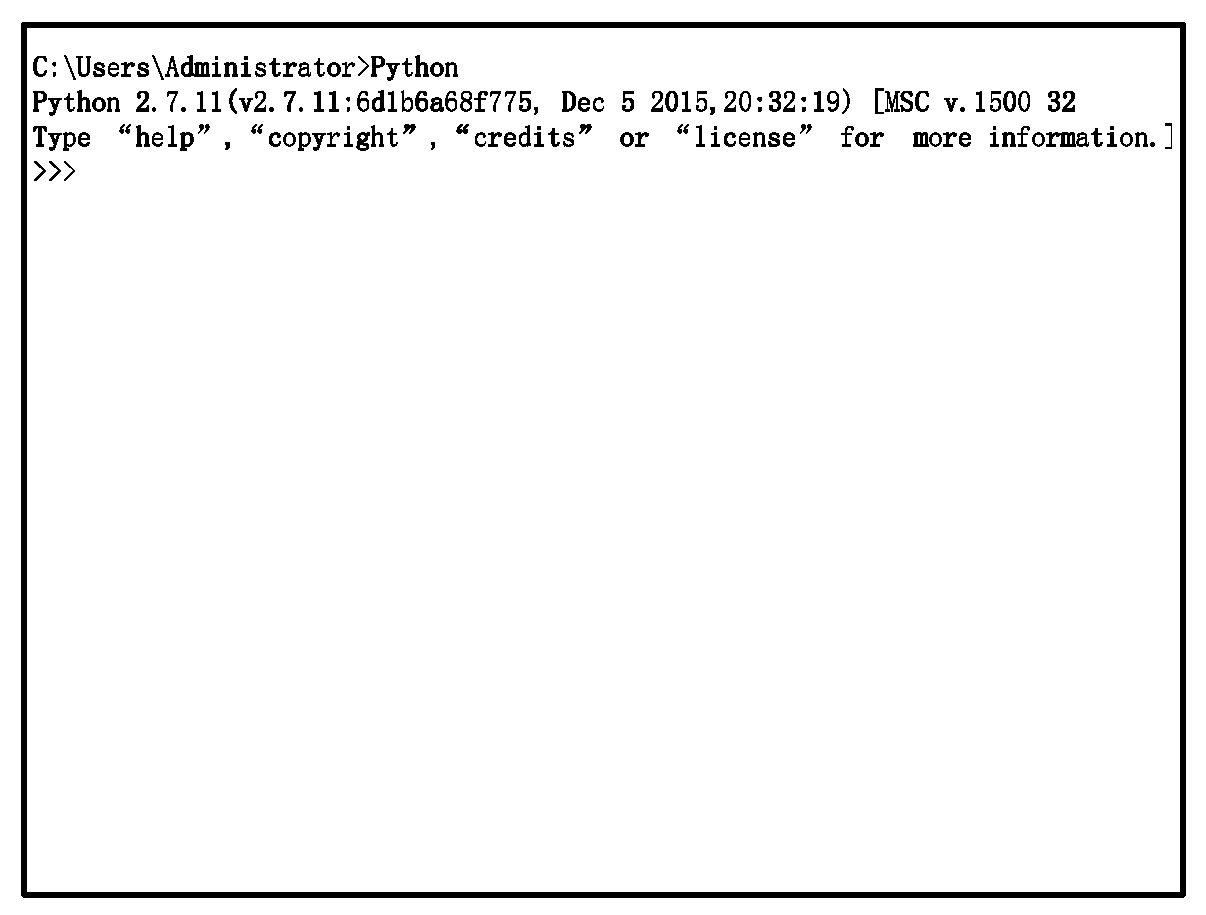
\includegraphics[width=10cm]{fig3_1}
%\caption{Python 安装勾选组件}
%\end{figure}
\begin{figure}[ht]
\centering
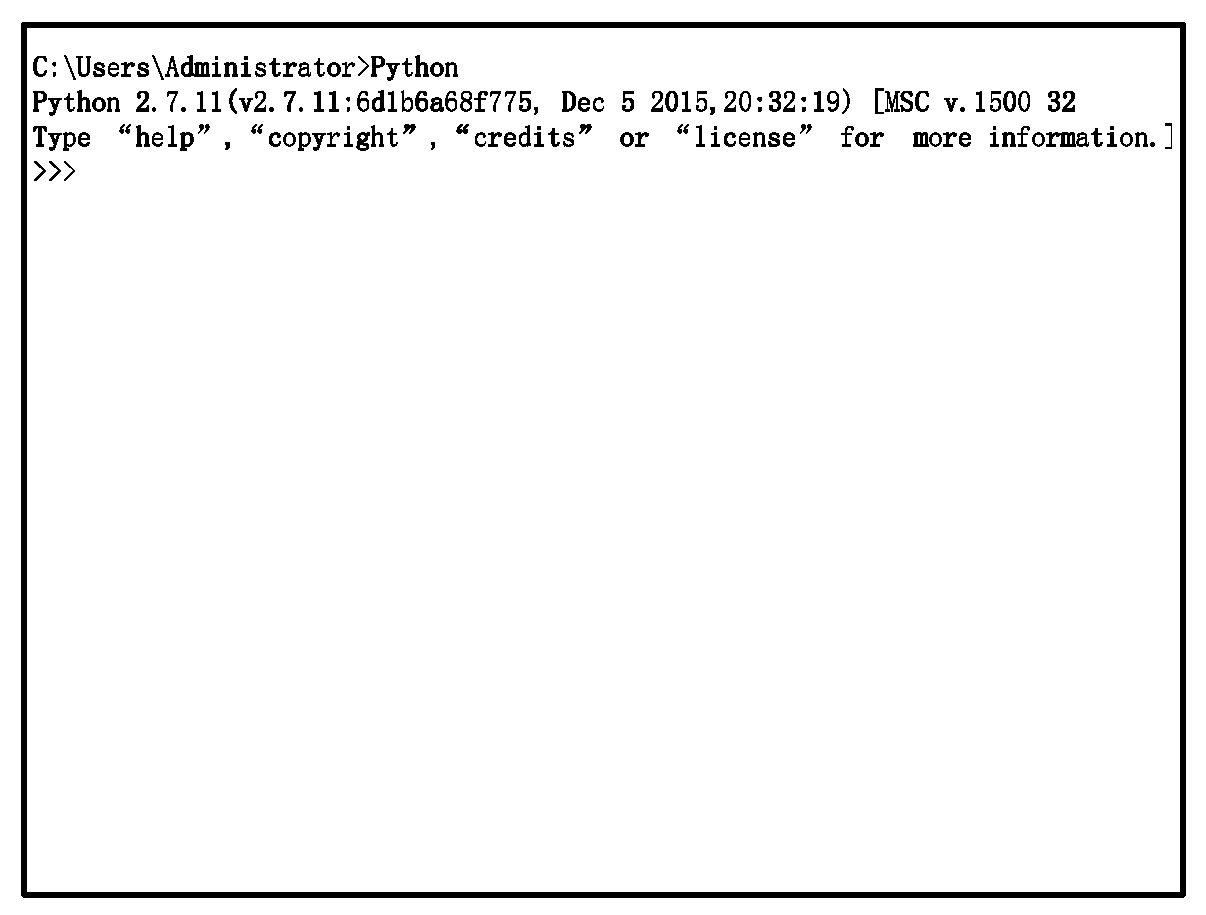
\includegraphics[width=11cm,height=8cm]{fig3_1}
\caption{Python 解释器安装成功}
\end{figure}

\section{Python\heiti 第三方库安装}
我司会为用户提供运行软件所需的所有第三方Python库的安装文件,包括wxpython、matplotlib(包括dateutil文件与pyparsing文件)、numpy、six等。下面依次讲解如何安装这4个第三方库。
\vspace{0.4cm}

\noindent$\vcenter{\hbox{\huge$\bullet$}}$\quad\fontsize{12pt}{\baselineskip}\textbf{\heiti{安装}wxpython\heiti{库}:}

进入我司为用户提供的“ASG\_install”文件夹下的wxpython文件夹,双击其中的exe安装程序,点击“Next”即可安装wxpython库。
\vspace{0.4cm}

\noindent$\vcenter{\hbox{\huge$\bullet$}}$\quad\fontsize{12pt}{\baselineskip}\textbf{\heiti{安装}matplotlib\heiti{库}:}

进入我司为用户提供的“ASG\_install”文件夹下的“matplotlib”文件夹,双击其中的exe安装程序,点击“Next”即可安装matplotlib库。安装matplotlib库后还需要安装两个文件:dateutil文件与pyparsing 文件。
\vspace{0.4cm}

\noindent$\vcenter{\hbox{\huge$\bullet$}}$\quad\fontsize{12pt}{\baselineskip}\textbf{\heiti{安装}dateutil\heiti{文件}:}

进入Windows命令行(点击任务栏“开始”按钮,输入“cmd”后按回车),然后通过DOS下的“cd”命令(切换目录),将当前目录切换到您存放我司提供的“matplotlib”文件夹所在位置。如用户将“ASG\_install”文件夹放在E盘的主目录下时,在命令窗口中依次输入“E:” → “cd ASG\_install” → “cd matplotlib”,即可将当前目录切换到存放“matplotlib”文件夹的位置。然后通过“pip install”命令来安装dateutil文件。完整过程为如图3.2,依次输入命令即可安装dateutil 文件。
\begin{figure}[ht]
\centering
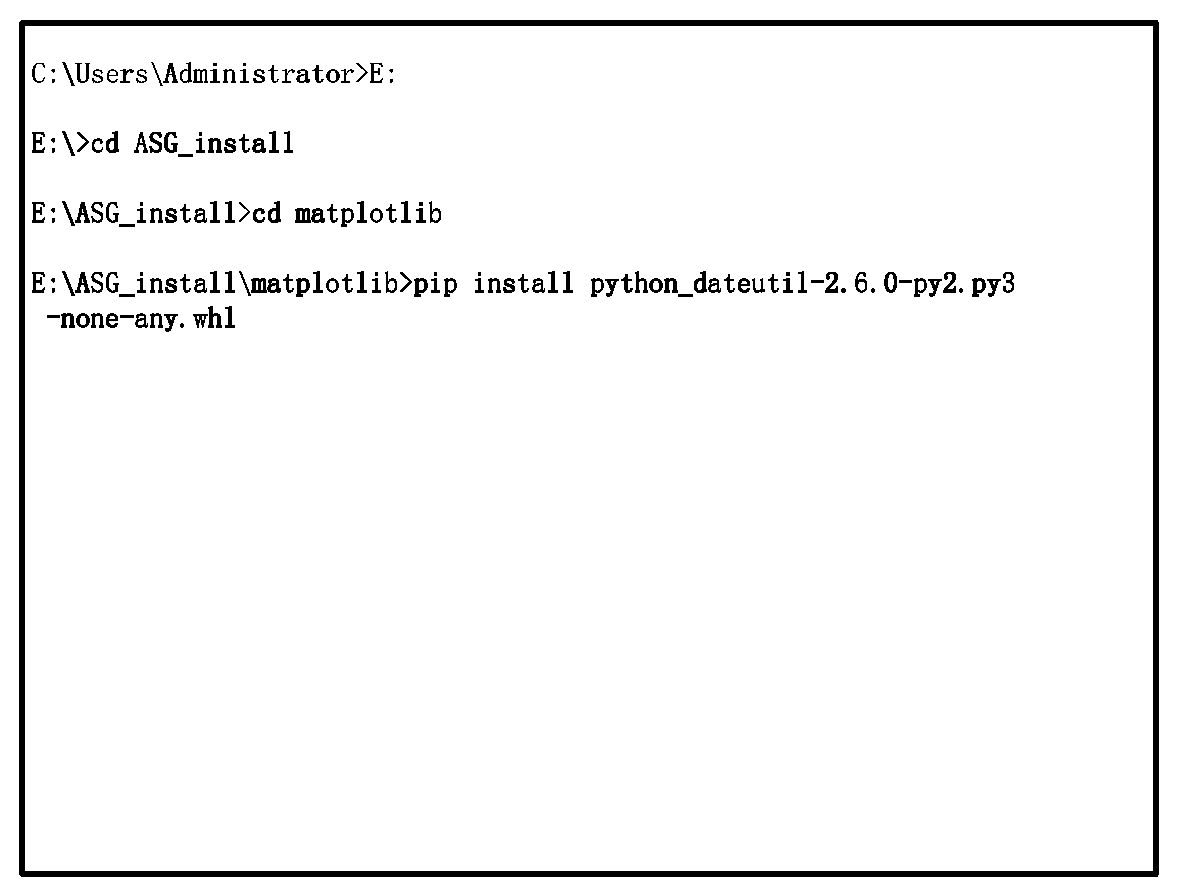
\includegraphics[width=11cm,height=8cm]{fig3_2}
\caption{安装dateutil文件}
\end{figure}

\newpage
\noindent$\vcenter{\hbox{\huge$\bullet$}}$\quad\fontsize{12pt}{\baselineskip}\textbf{\heiti{安装}pyparsing\heiti{文件}:}

同安装dateutil一样,先在DOS命令窗口将目录切换到我司提供的“matplotlib”文件夹所在位置,然后通过“pip install”命令来安装pyparsing文件。如用户将“ASG\_install”文件夹放在E盘的主目录下时,完整安装过程如图3.3。

%进入Windows命令行,然后将目录切换到您存放我司提供的“matplotlib”文件夹所在位置。如图3-3输入命令即可安装pyparsing文件。

\begin{figure}[H]
\centering
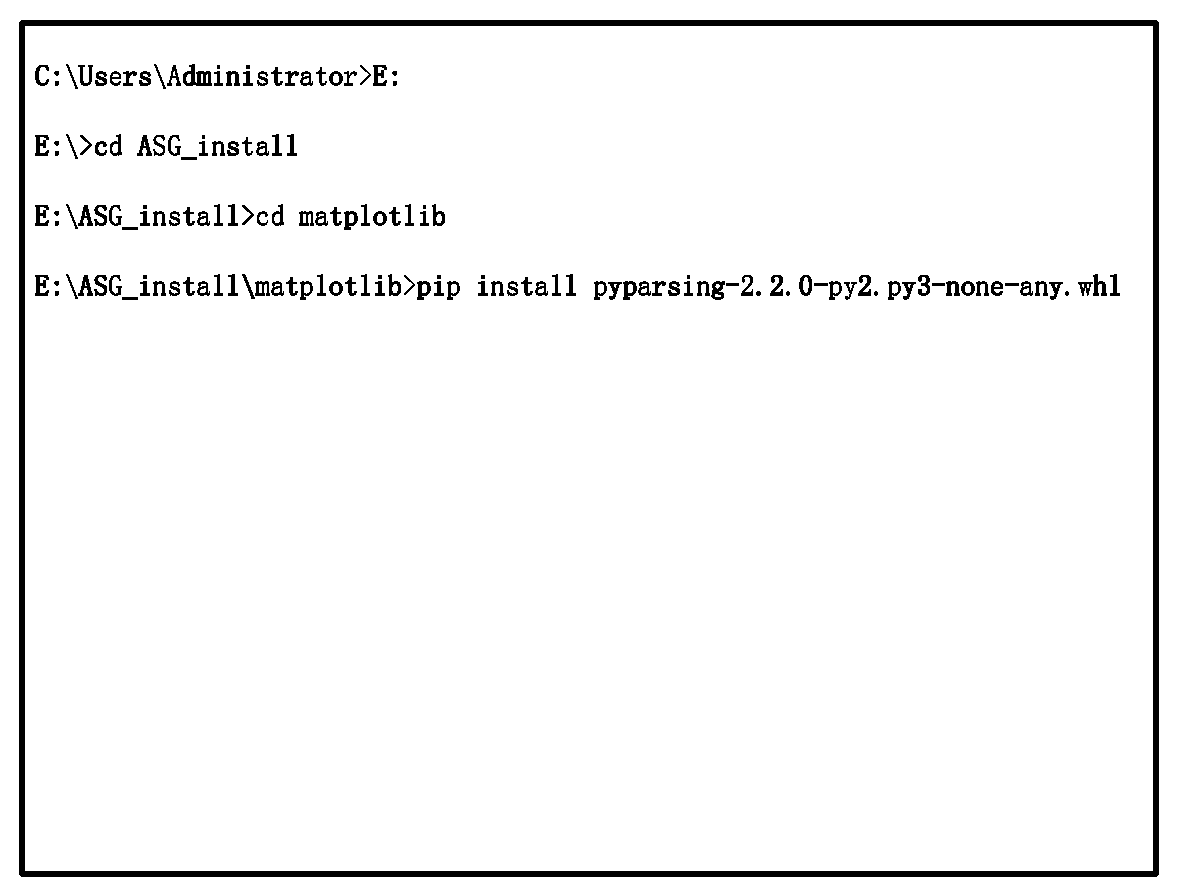
\includegraphics[width=11cm,height=8cm]{fig3_3}
\caption{安装pyparsing文件}
\end{figure}

\noindent$\vcenter{\hbox{\huge$\bullet$}}$\quad\fontsize{12pt}{\baselineskip}\textbf{\heiti{安装}numpy\heiti{库}:}

在DOS命令窗口将目录切换到存放我司提供的“numpy”文件夹所在位置,然后通过“pip install”命令来安装numpy库。如用户将“ASG\_install”文件夹放在E盘的主目录下时,完整安装过程如图3.4。
\begin{figure}[H]
\centering
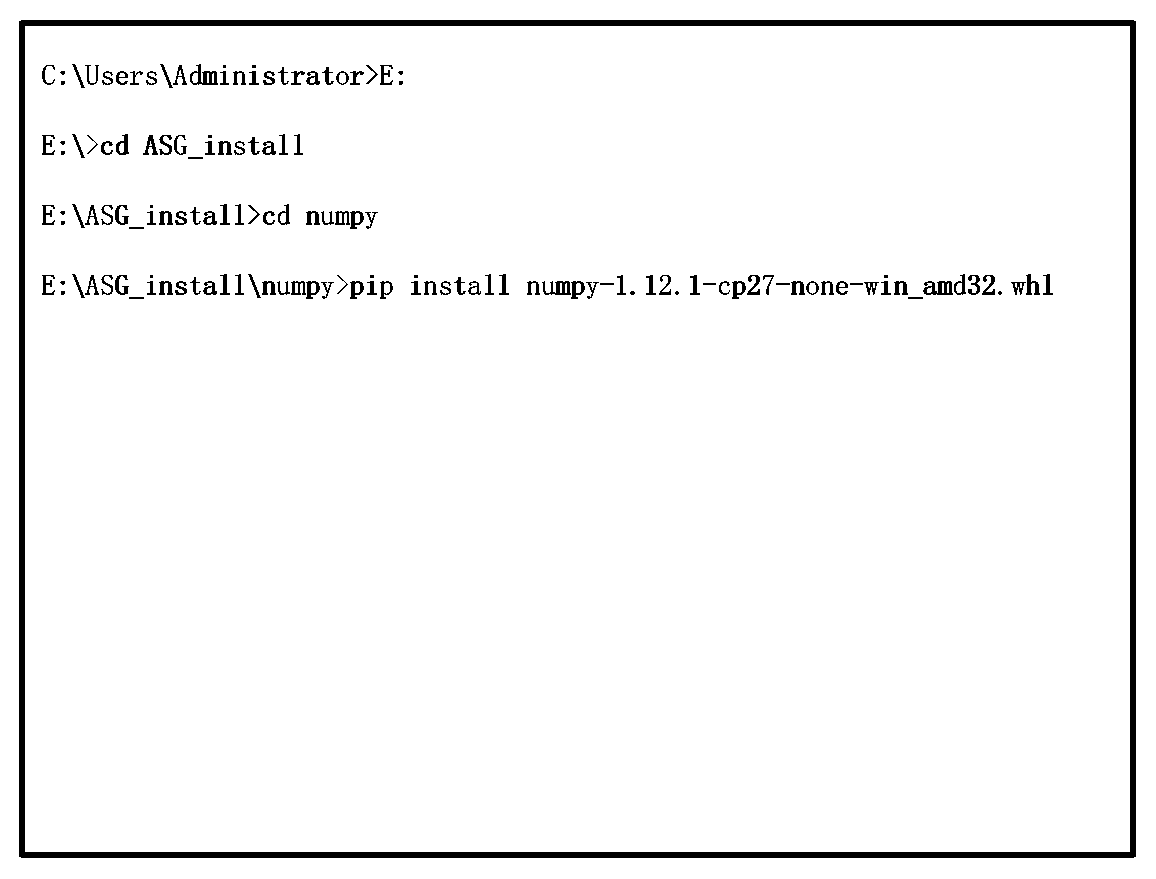
\includegraphics[width=11cm,height=8cm]{fig3_4}
\caption{安装numpy库}
\end{figure}

\noindent$\vcenter{\hbox{\huge$\bullet$}}$\quad\fontsize{12pt}{\baselineskip}\textbf{\heiti{安装}six\heiti{库}:}

在DOS命令窗口将目录切换到存放我司提供的“six”文件夹所在位置,然后通过“pip install”命令来安装six库。如用户将“ASG\_install”文件夹放在E盘的主目录下时,完整安装过程如图3.5。
%进入Windows命令行,然后将目录切换到您存放我司提供的“six”文件夹所在位置。如图3-5输入命令即可安装six库。
\begin{figure}[H]
\centering
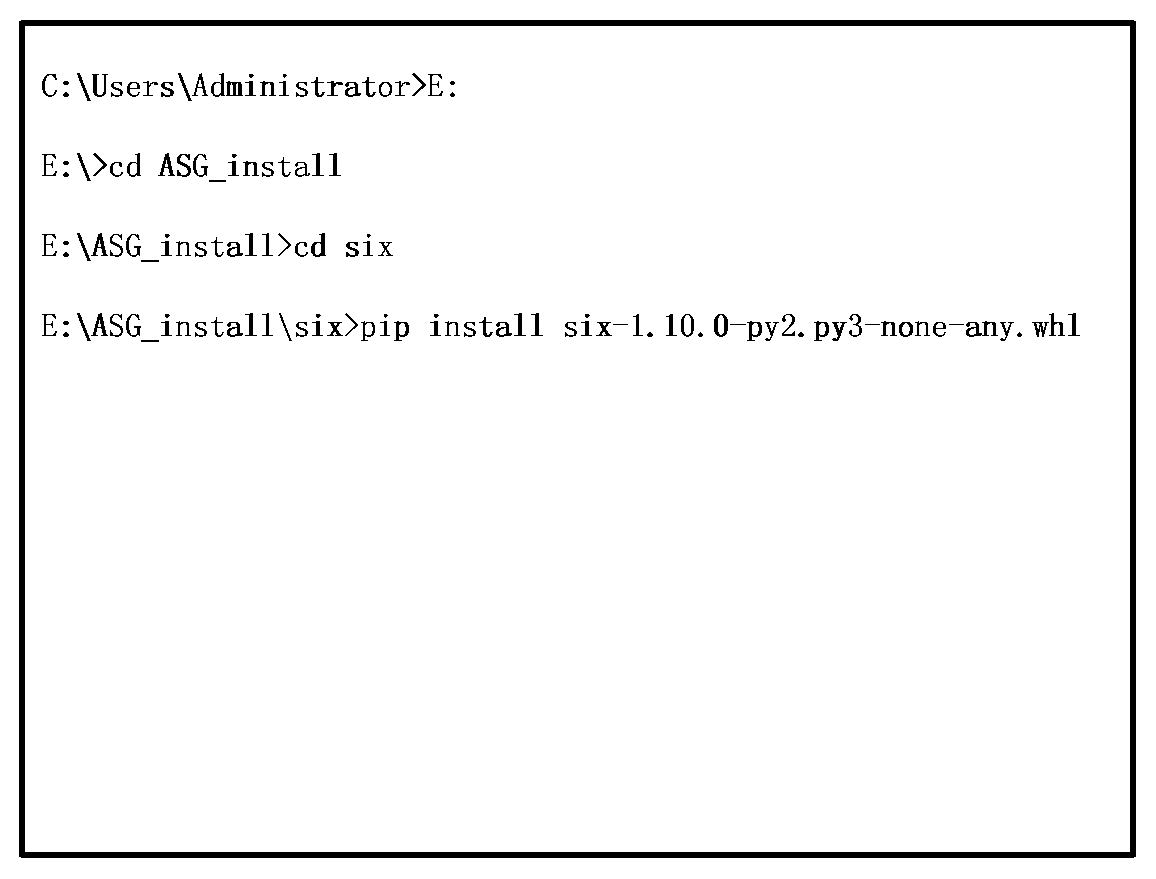
\includegraphics[width=11cm,height=8cm]{fig3_5}
\caption{安装six库}
\end{figure}

\section{USB\heiti 驱动程序安装}
在一台计算机上首次连接仪器时,系统会自动安装仪器运行所需的USB驱动程序。若自动安装失败,请打开计算机设备管理器,在“通用串行总线控制器”找到驱动未安装成功的设备,手动安装驱动程序(右键选择设备→ 更新驱动程序软件→浏览计算机以查找驱动程序软件),定位至我司为用户提供的“Drivers”文件夹即可。驱动安装成功后,在设备管理器中可以看到如图3.6所示的“Cypress FX3 USB StreamerExample Device” 被识别的状态。
\begin{figure}[htbp]
\centering
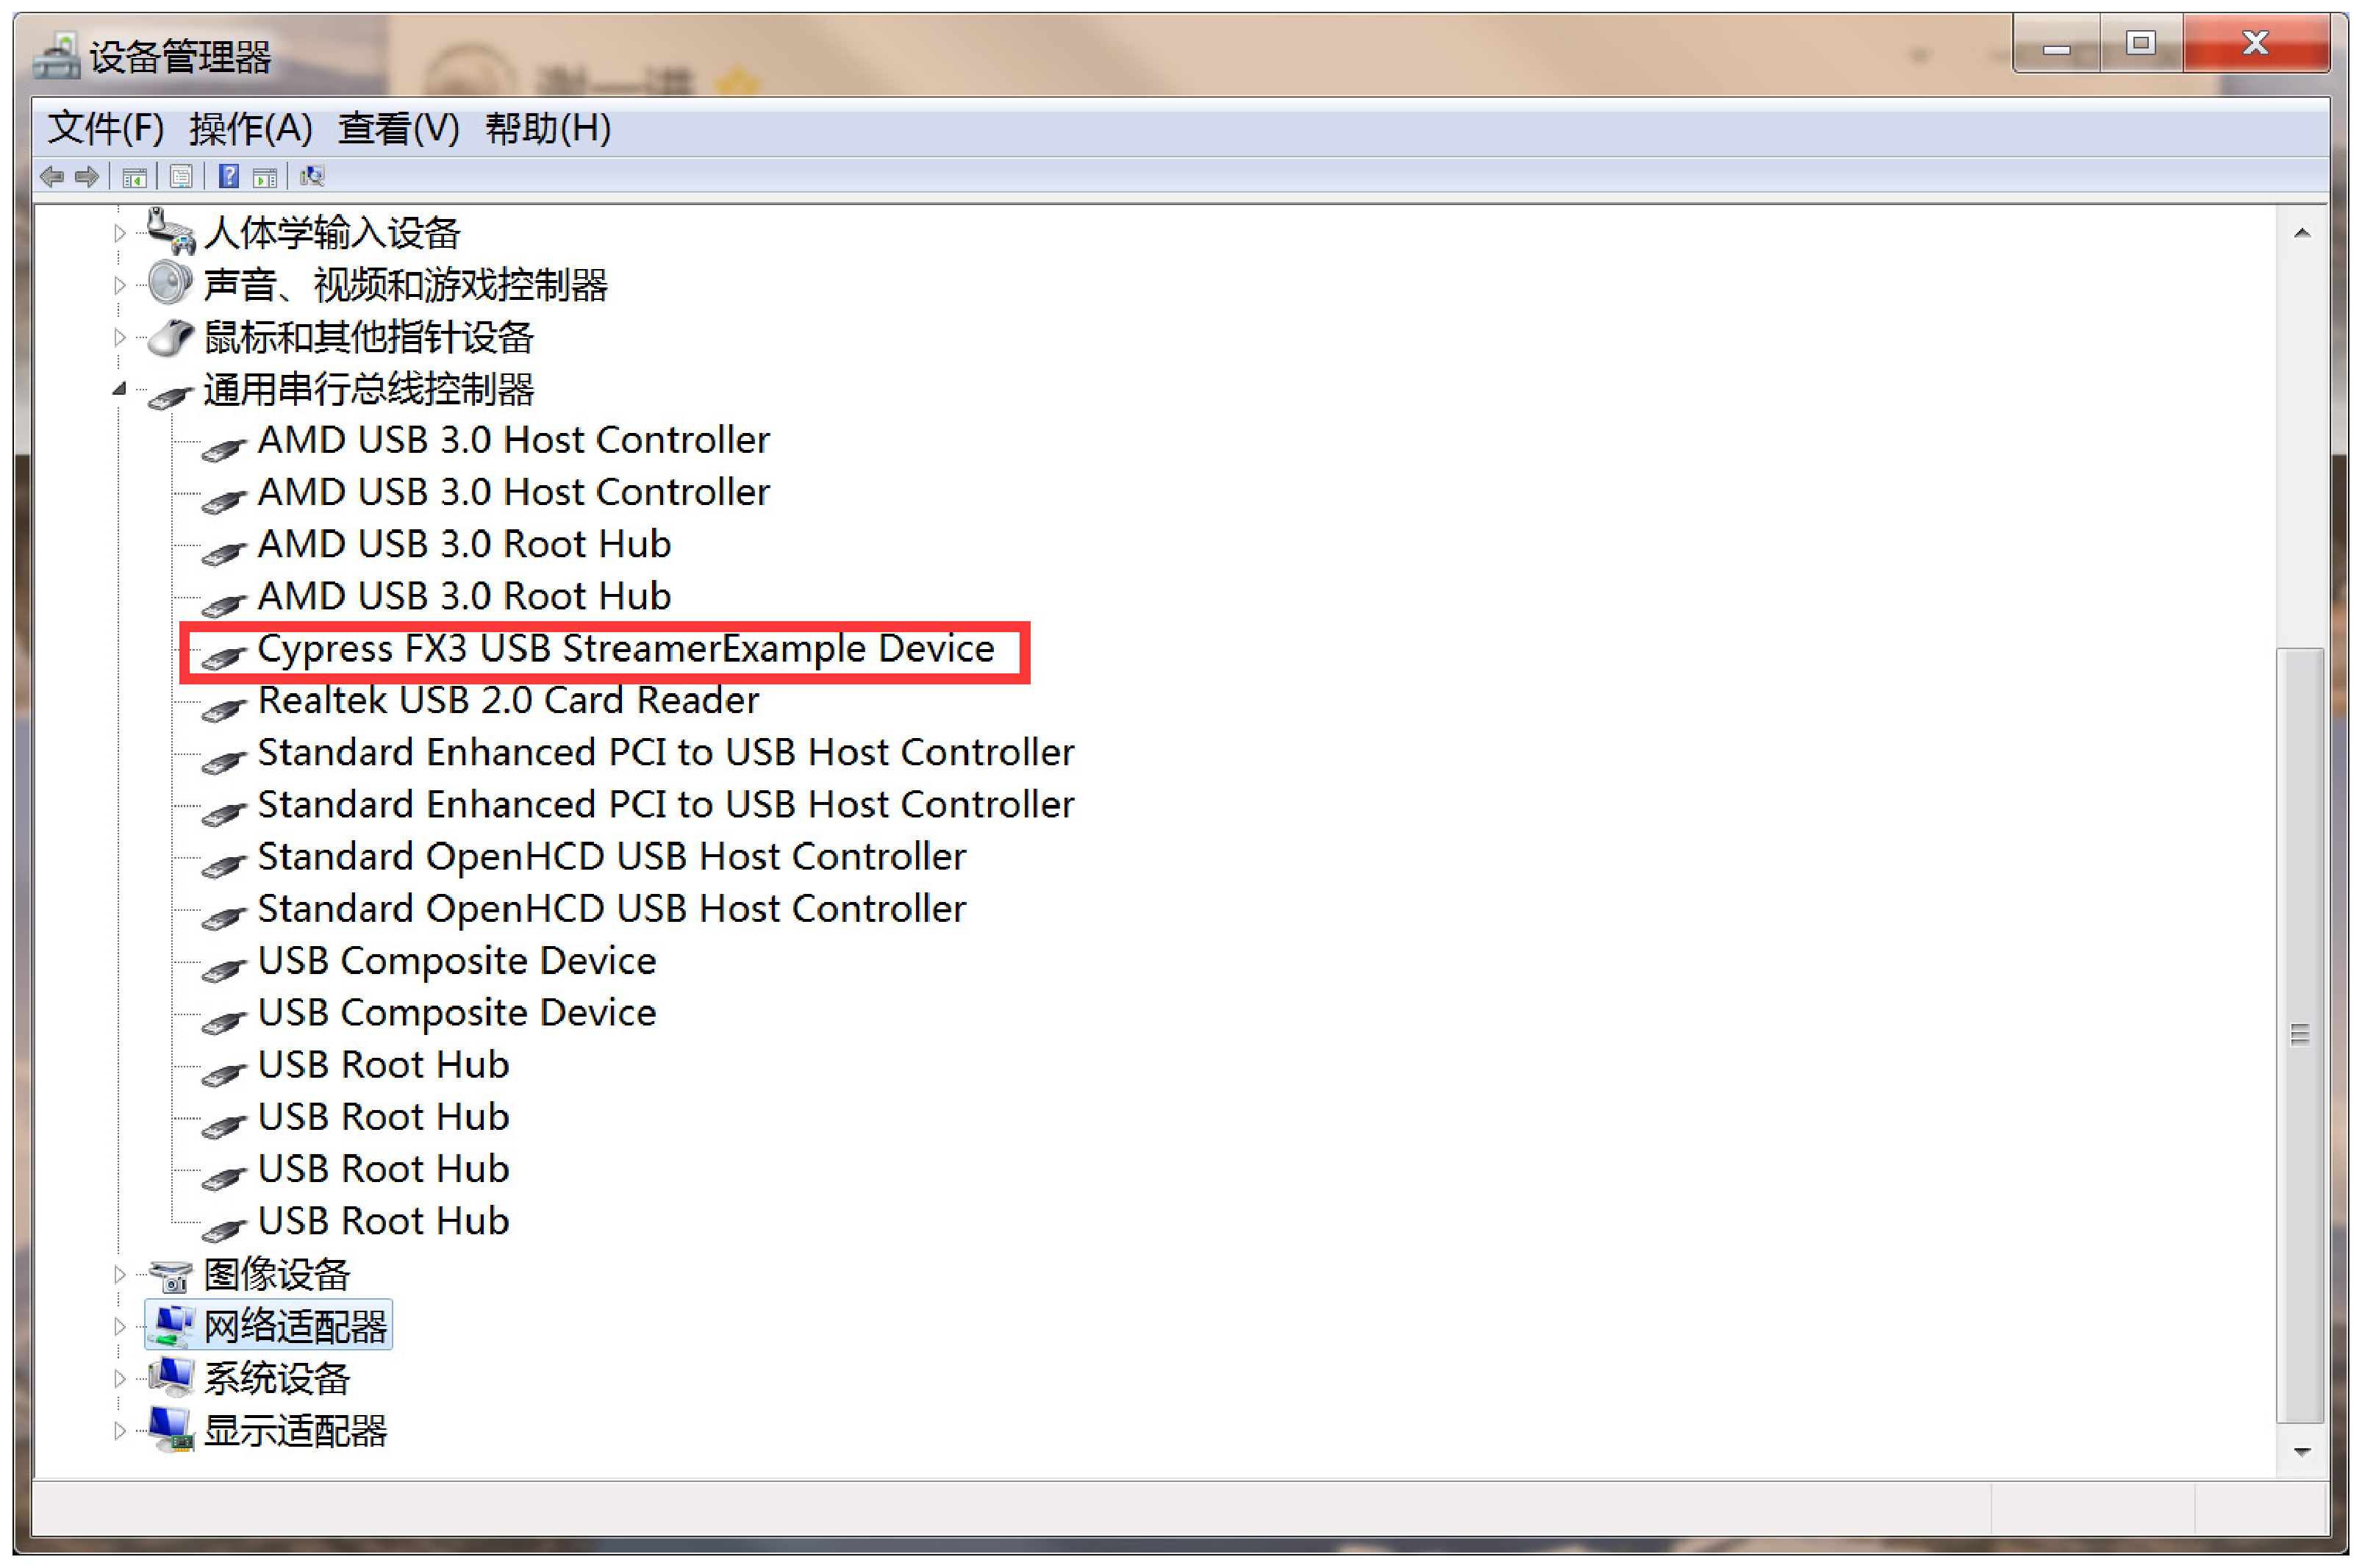
\includegraphics[width=10cm,height= 8.0cm]{fig3_6}
\caption{驱动程序安装}
\end{figure}

驱动程序安装完成后,双击“Cypress FX3 USB StreamerExample Device”打开其属性,进入“电源管理”选项。如图3.7,取消勾选“允许计算机关闭此设备以节约电源”。
\begin{figure}[htbp]
\centering
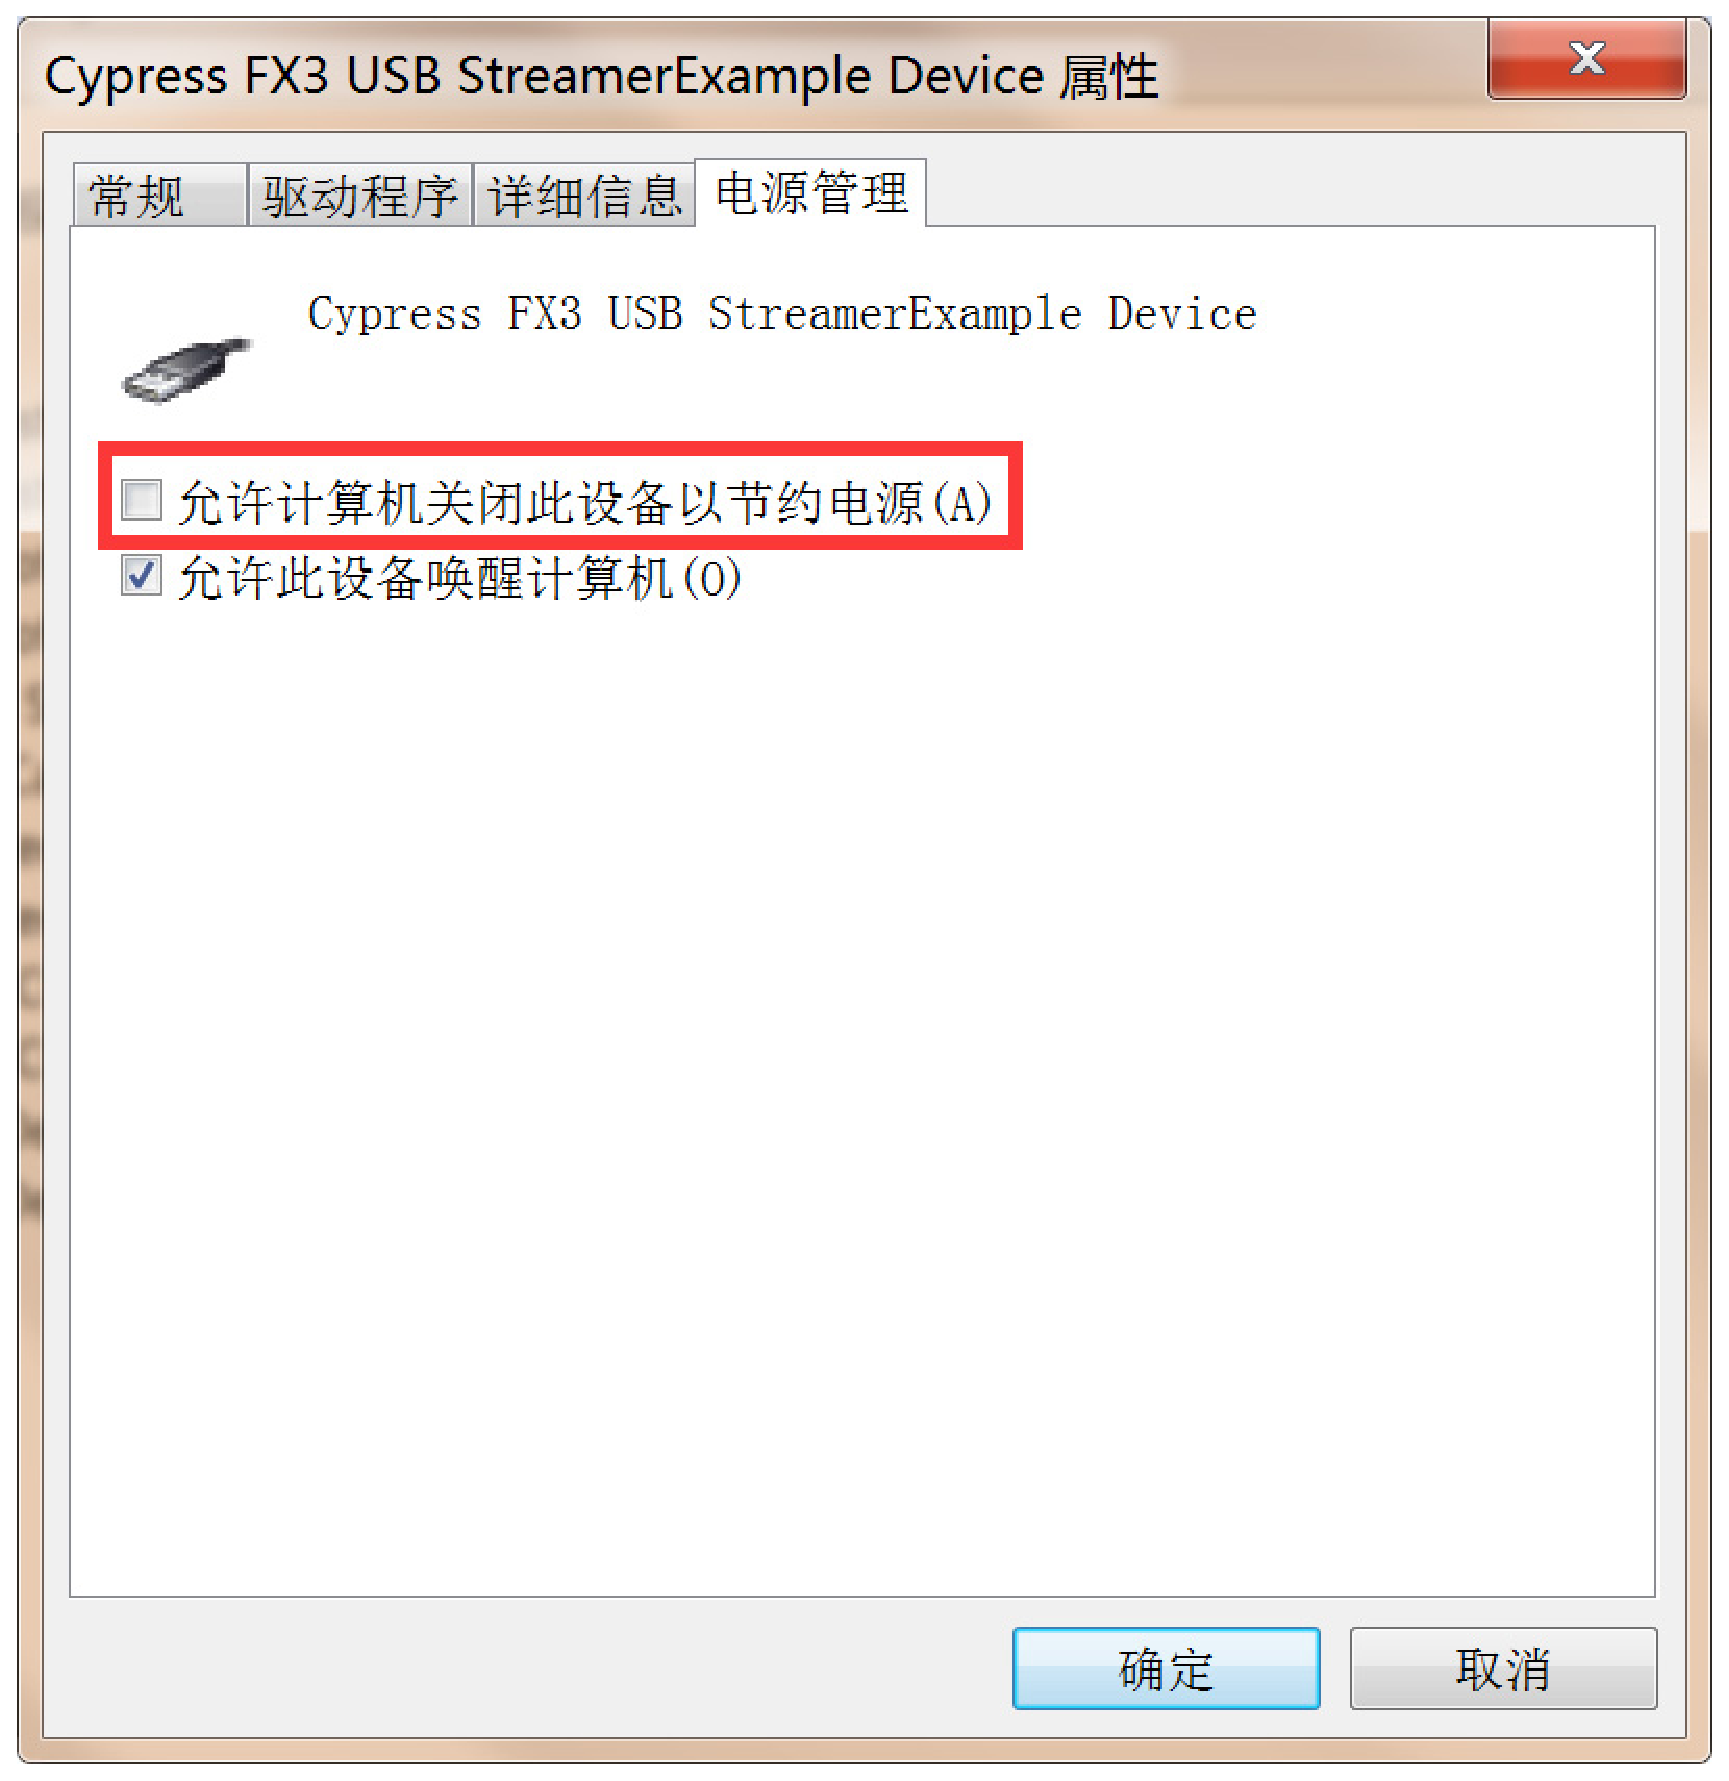
\includegraphics[width=10cm,height=8.5cm]{fig3_7}
\caption{更改电源管理选项}
\end{figure}





\chapter{\heiti 软件使用}
\section{\heiti 打开控制软件}
进入我司为用户提供的Integration的文件夹,双击运行“ASG.py”文件,即可打开方波序列编辑软件。软件主界面(Pulse界面)如图4.1所示。
\begin{figure}[ht]
\centering
%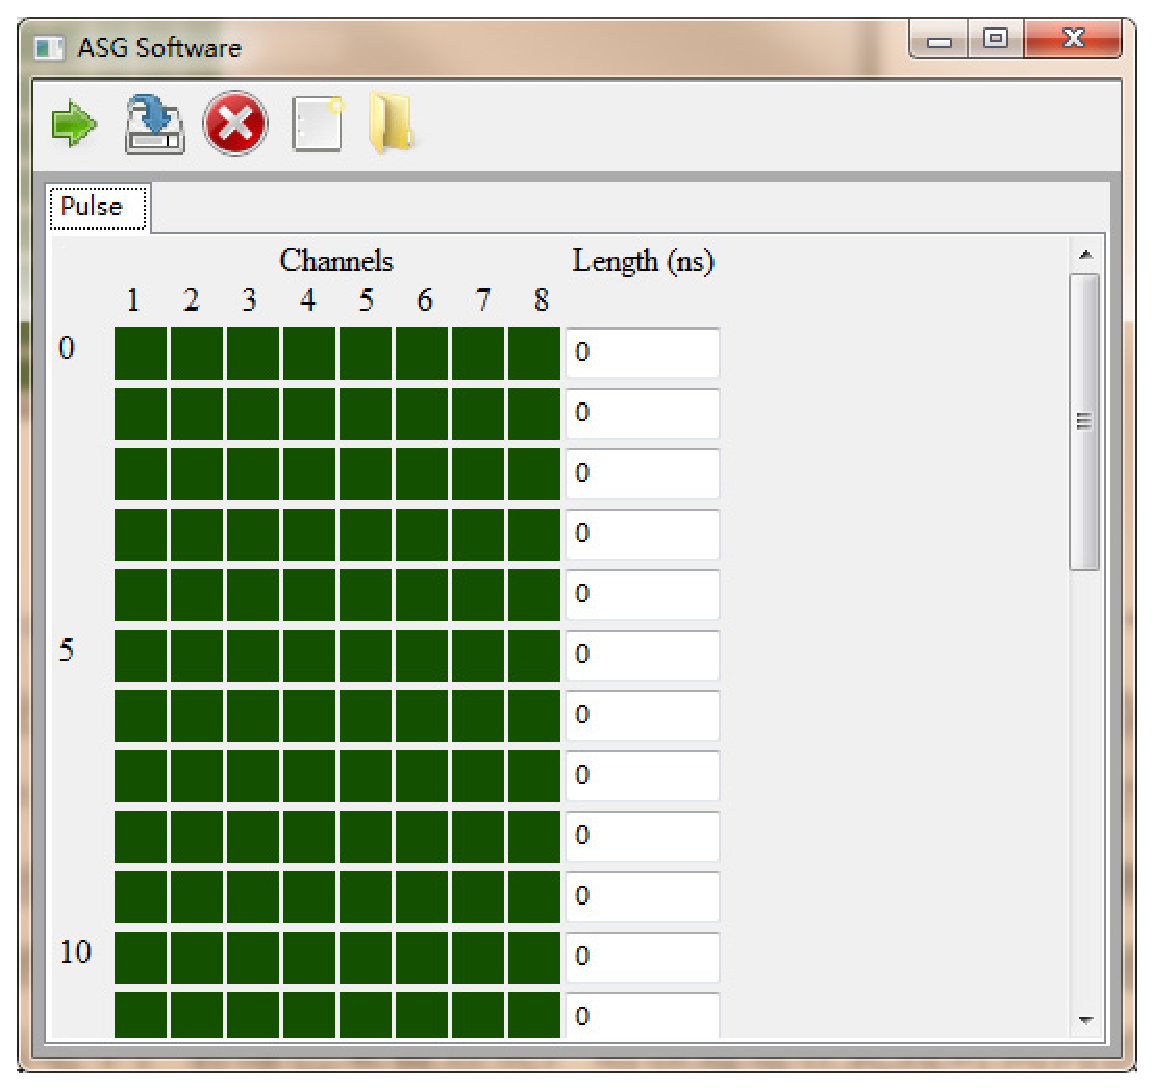
\includegraphics[width=11cm,height=9cm]{fig4_1}
%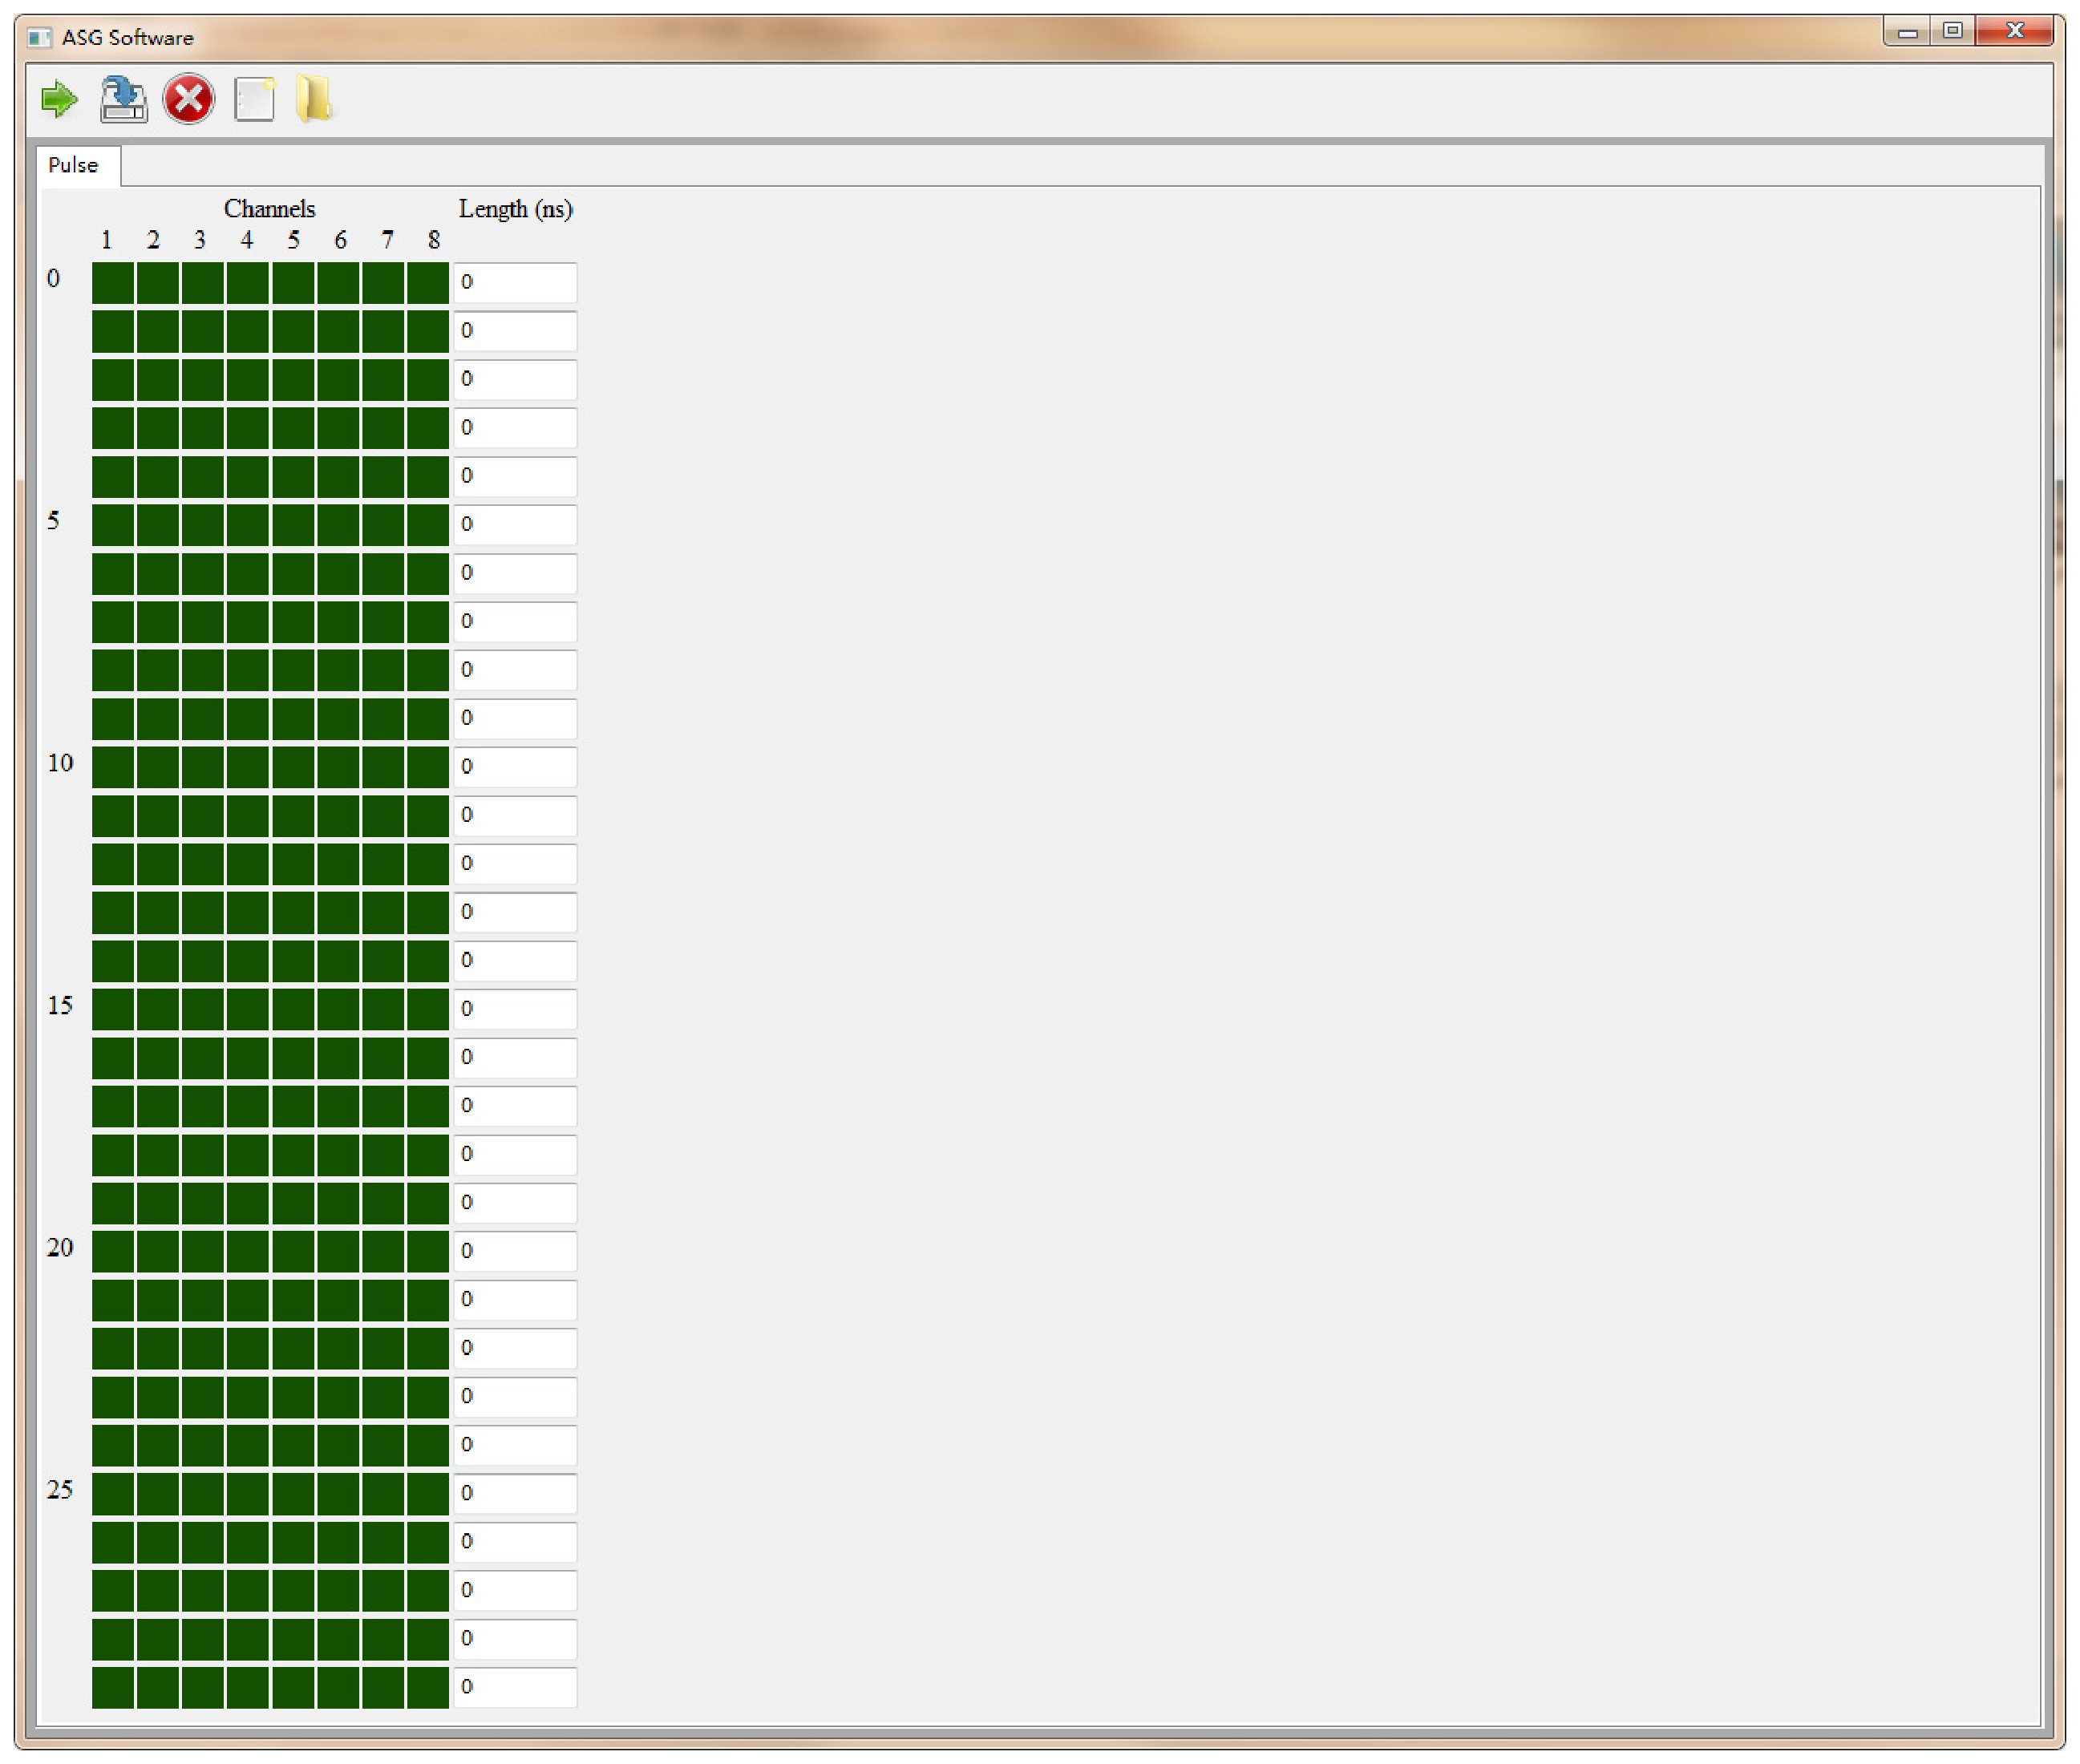
\includegraphics[width=12cm,height=9cm]{fig4_1_xyj}
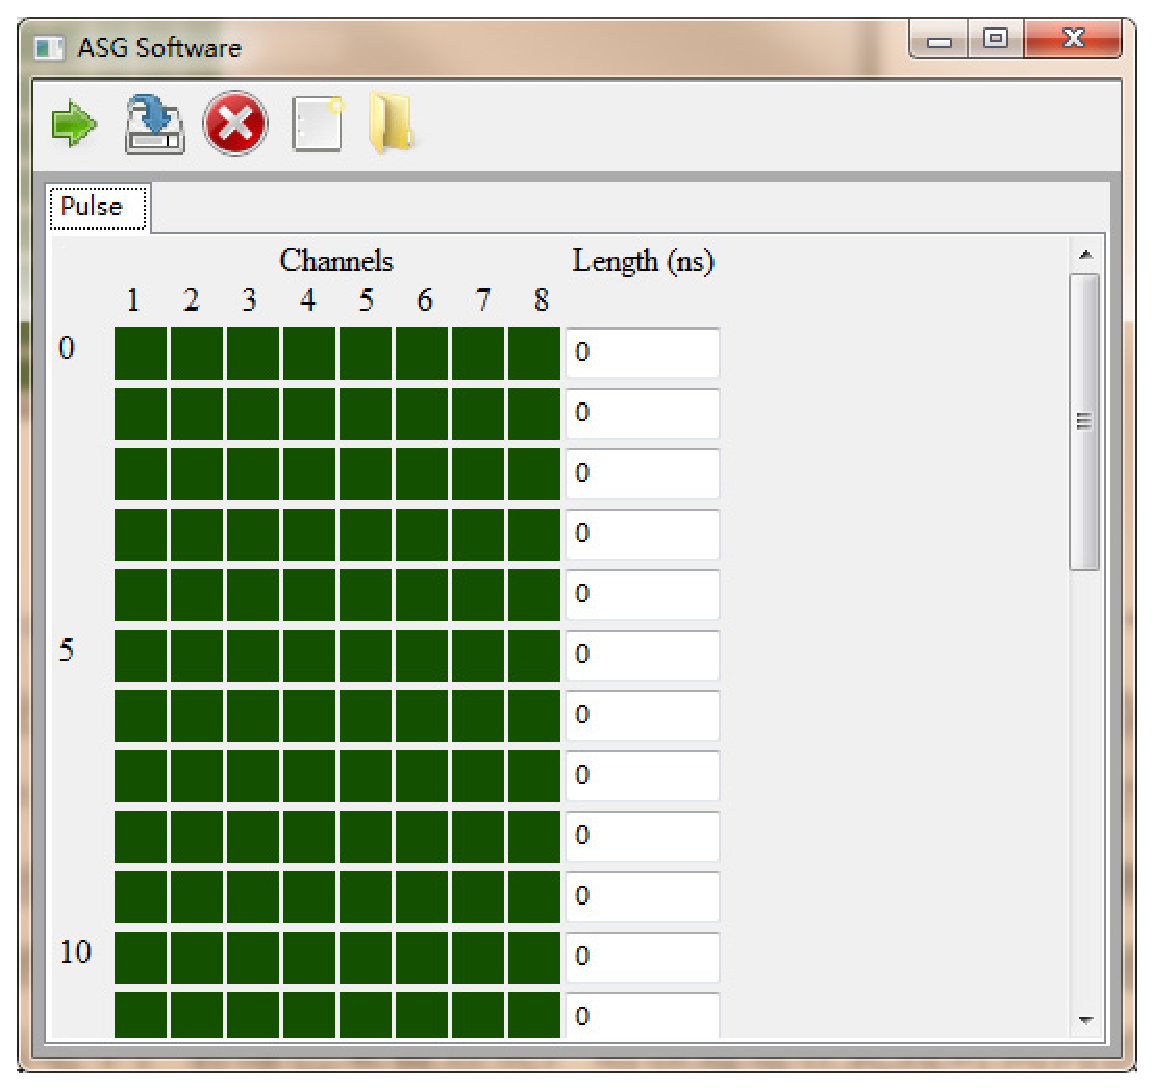
\includegraphics[height=9cm]{fig4_1}
\caption{软件主界面}
\end{figure}

在软件主界面工具栏中,从左往右5个按钮依次为:“开始播放按钮”、“下载方波数据按钮”、“停止播放按钮”、“存储当前方波序列按钮”、“载入存储方波序列按钮”。界面中间的每行8个绿色方框,从左往右依次代表OUT 1 至OUT 8 的8 个方波输出通道在一段时间内的输出状态(时间长度由右侧的“Length” 文本框内输入的数值决定,单位为纳秒)。当绿色被点亮时,该通道在此段时间内的输出为高电平;若绿色未被点亮,则该通道在此段时间内的输出为低电平。

\section{\heiti 定义任意方波序列举例}
用户可根据每行绿色方框的不同状态及“Length”的长度来定义任意的方波序列。如图4.2,左侧“CH - 1”至“CH - 4”代表4个方波输出通道,若用户想要生成如图4.2所示的方波序列,可如图4.3在软件界面中定义该方波序列。

\newpage
\vspace{0.6cm}
\begin{figure}[H]
\centering
%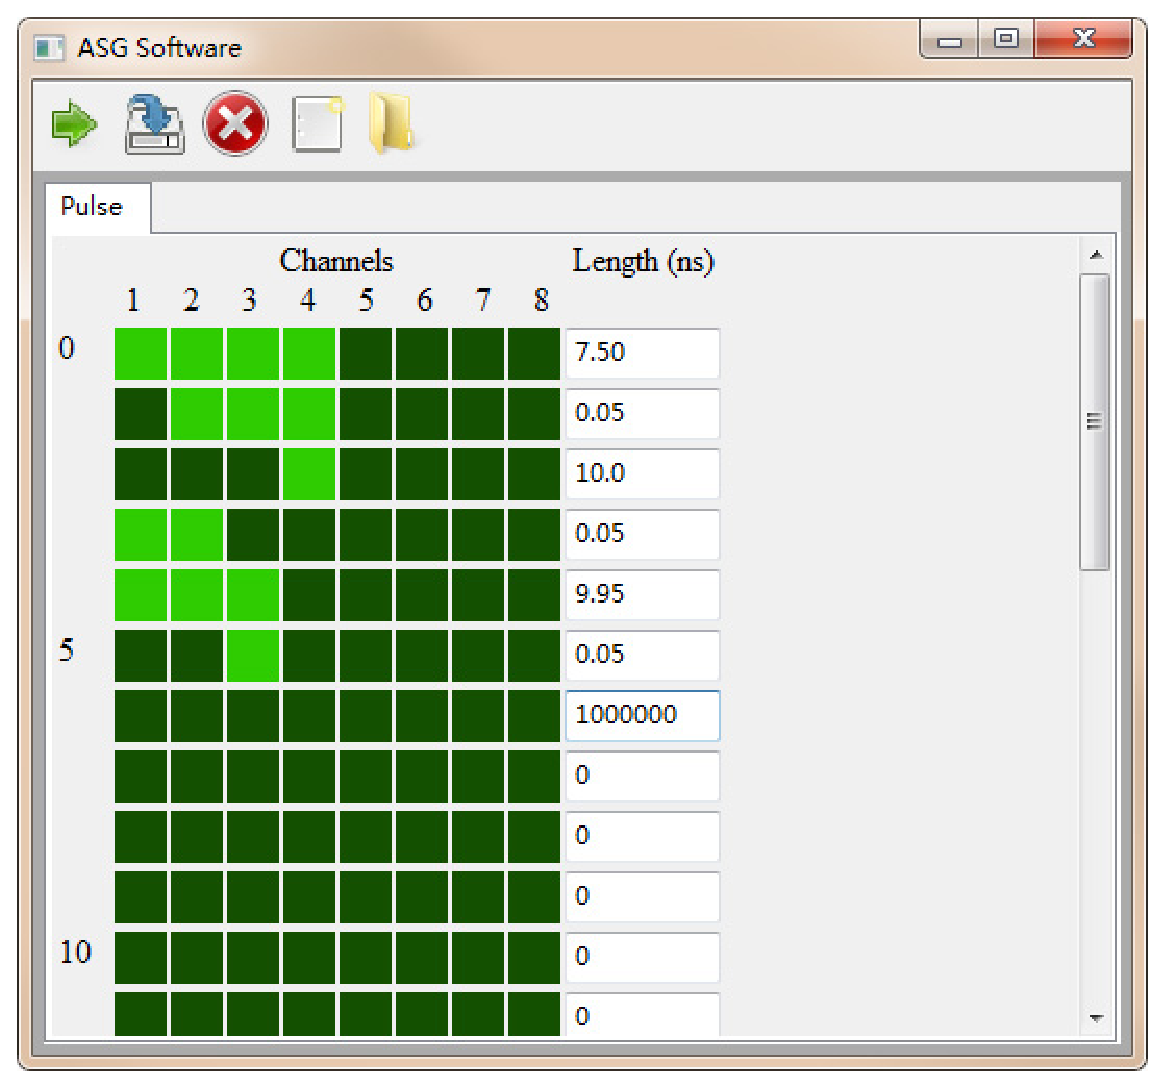
\includegraphics[width=11cm,height=9cm]{fig4_2}
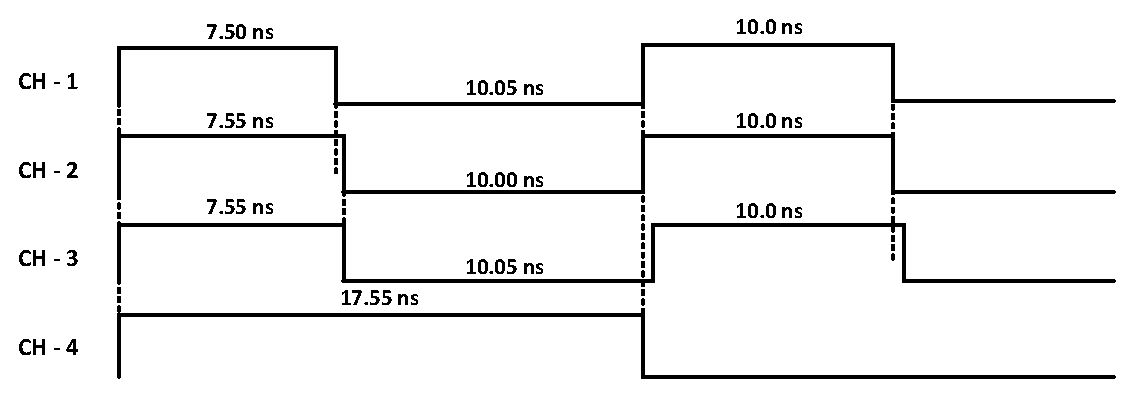
\includegraphics[height=5cm,width=14cm]{fig4_2_shixutu}
\caption{自定义方波序列时序图}
\end{figure}

\vspace{1cm}
\begin{figure}[H]
\centering
%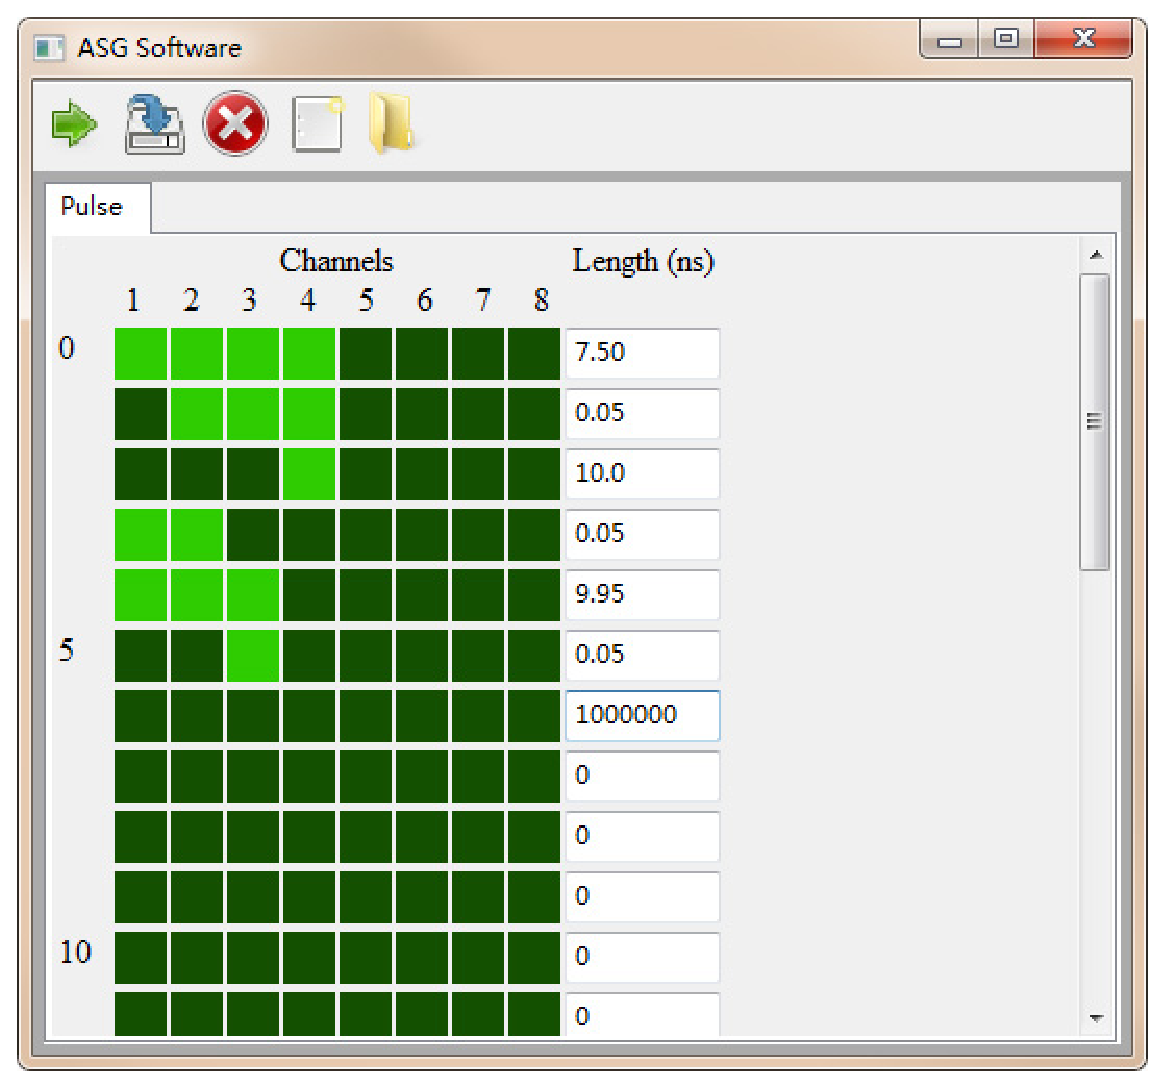
\includegraphics[width=11cm,height=9cm]{fig4_2}
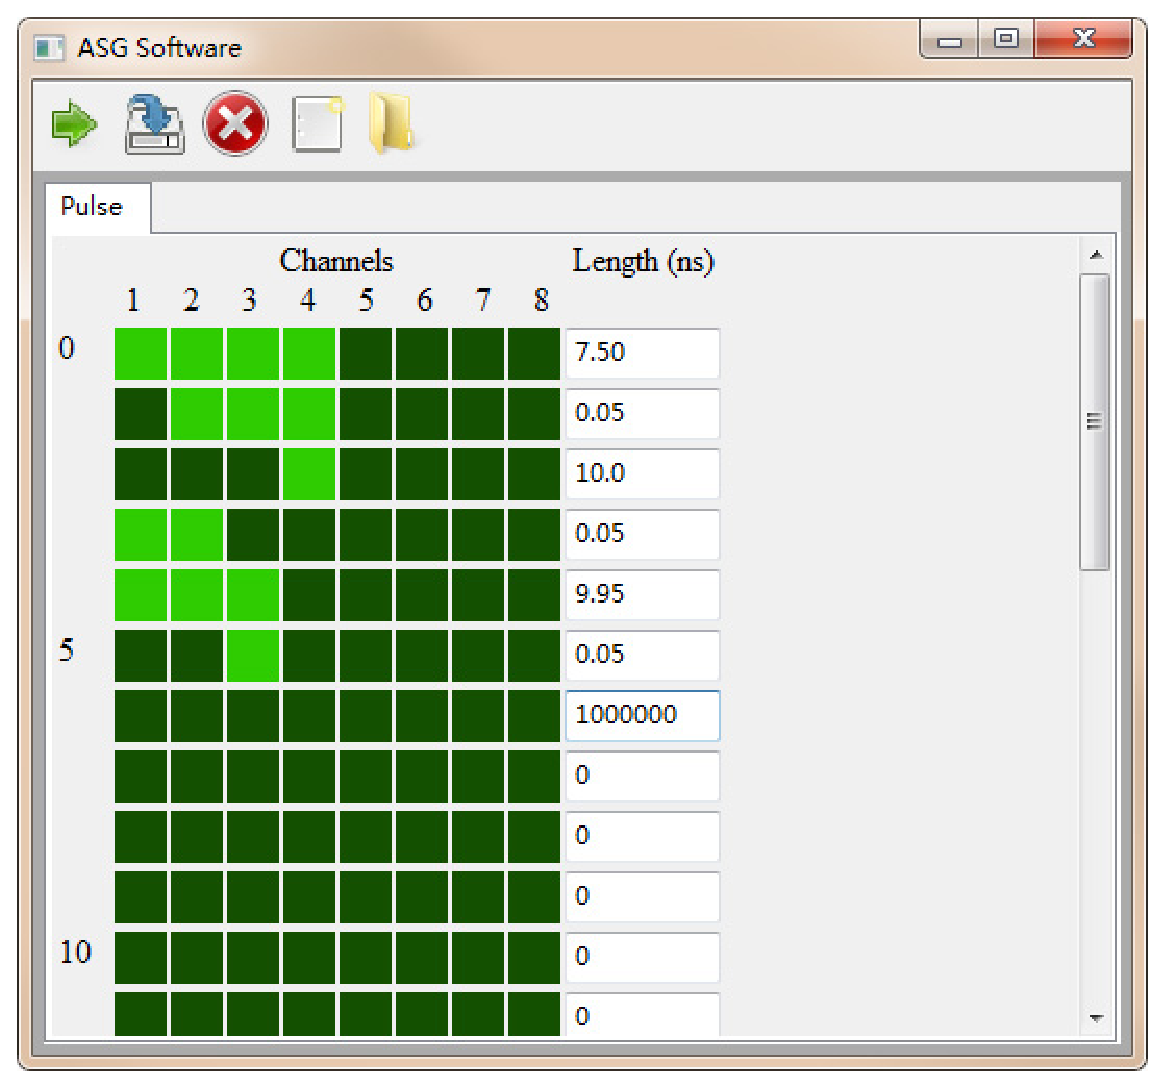
\includegraphics[height=9cm]{fig4_2}
\caption{使用软件定义方波序列}
\end{figure}
\vspace{0.6cm}
如图4.3使用方波编辑软件定义图4.2中的方波序列,这里只使用了4个方波输出通道,若用户需要同时使用更多的方波输出通道,可用同样的方法在其他通道定义任意方波序列。

\newpage
\section{\heiti 开始播放方波序列}
用户点击“Download”按钮
\includegraphics[height=0.7cm]{download},可将自定义的方波序列数据下载到硬件中。点击“Start”按钮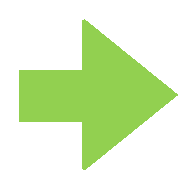
\includegraphics[height=0.7cm]{start},可使仪器各输出通道开始播放用户自定义的方波序列,在点击“Start” 按钮之前必须先将方波序列数据下载到硬件中。将输出通道用同轴线连接至示波器上可以看到仪器输出的方波波形。如用户定义图4.2所示方波序列,在示波器上可以看到如图4.4 所示的方波序列。

\vspace{2cm}

\begin{figure}[htbp]
\centering
%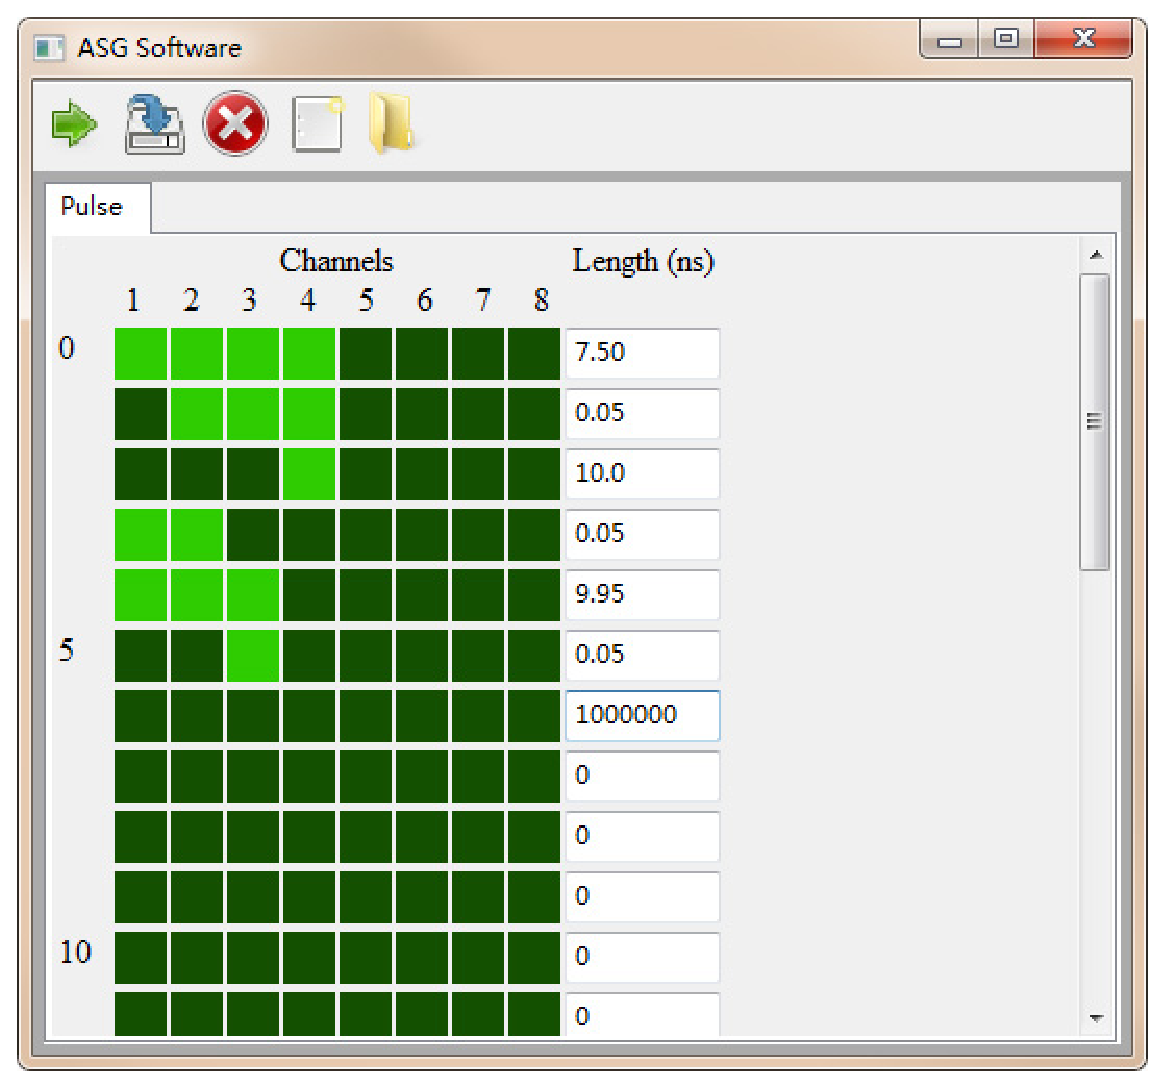
\includegraphics[width=11cm,height=9cm]{fig4_2}
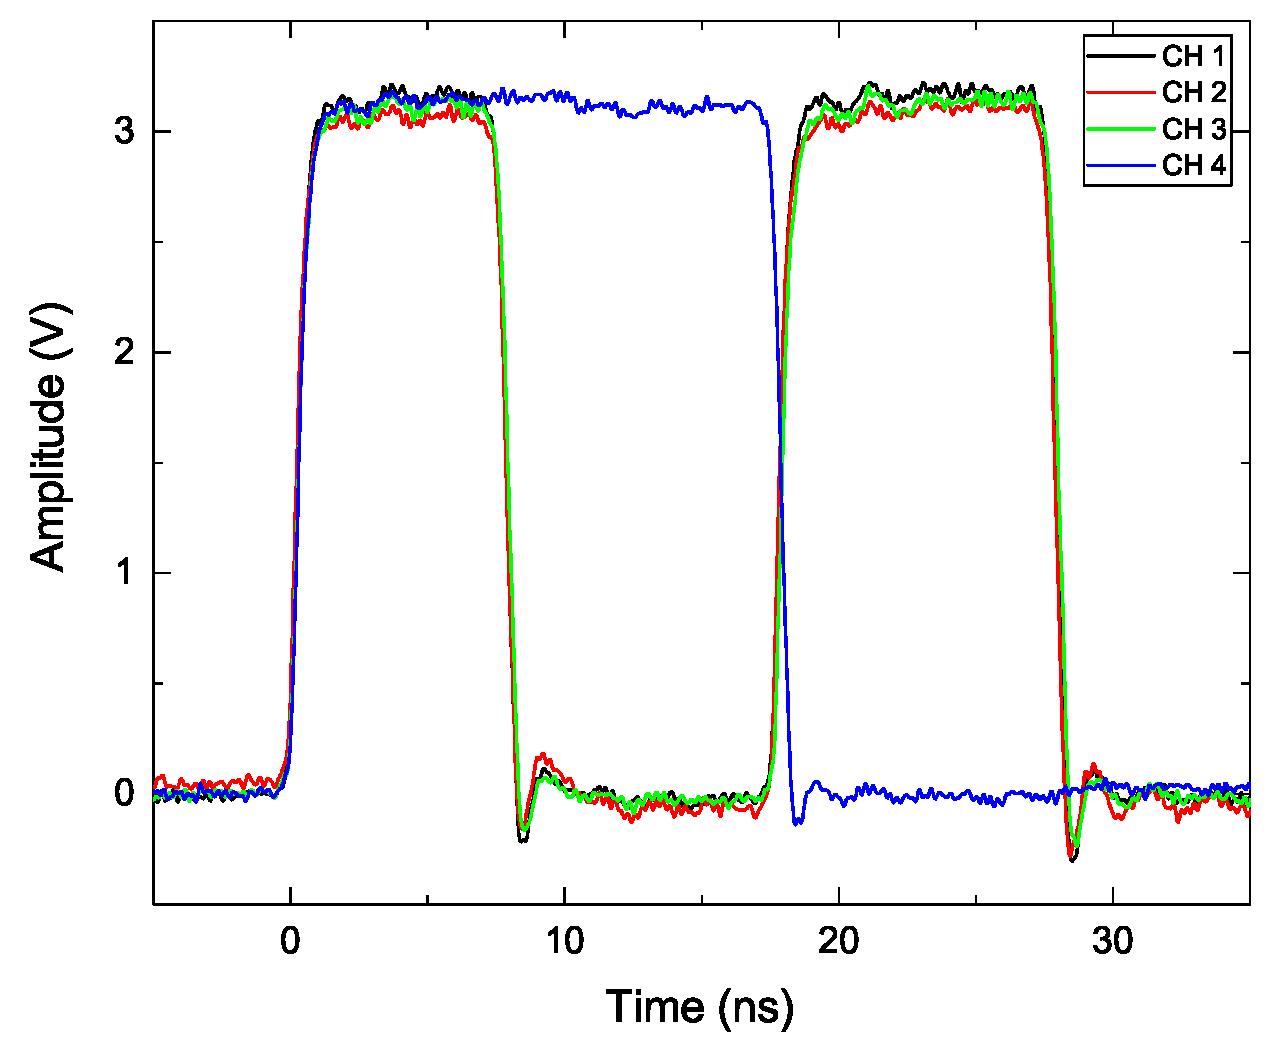
\includegraphics[height=9cm]{yangheng_shiboqi}
\caption{产品输出方波序列图}
\end{figure}


\section{\heiti 停止播放方波序列}
当仪器正在播放方波序列时,可以通过点击“Stop”按钮
\includegraphics[height=0.7cm]{stop}使仪器停止播放方波序列。


\newpage
\section{\heiti 定义方波序列注意事项}

\vspace{0.4cm}
\noindent \textbf{(1)}. 每个通道的方波序列中单个方波脉冲的高低电平时间必须在7.5 ns至2.6 s以内。如图4.5,当用户定义的方波序列中单个脉冲宽度小于7.5 ns 时,软件会弹出提示对话框让用户检查自定义的方波序列是否符合要求。

\vspace{0.2cm}
\begin{figure}[H]
\centering
%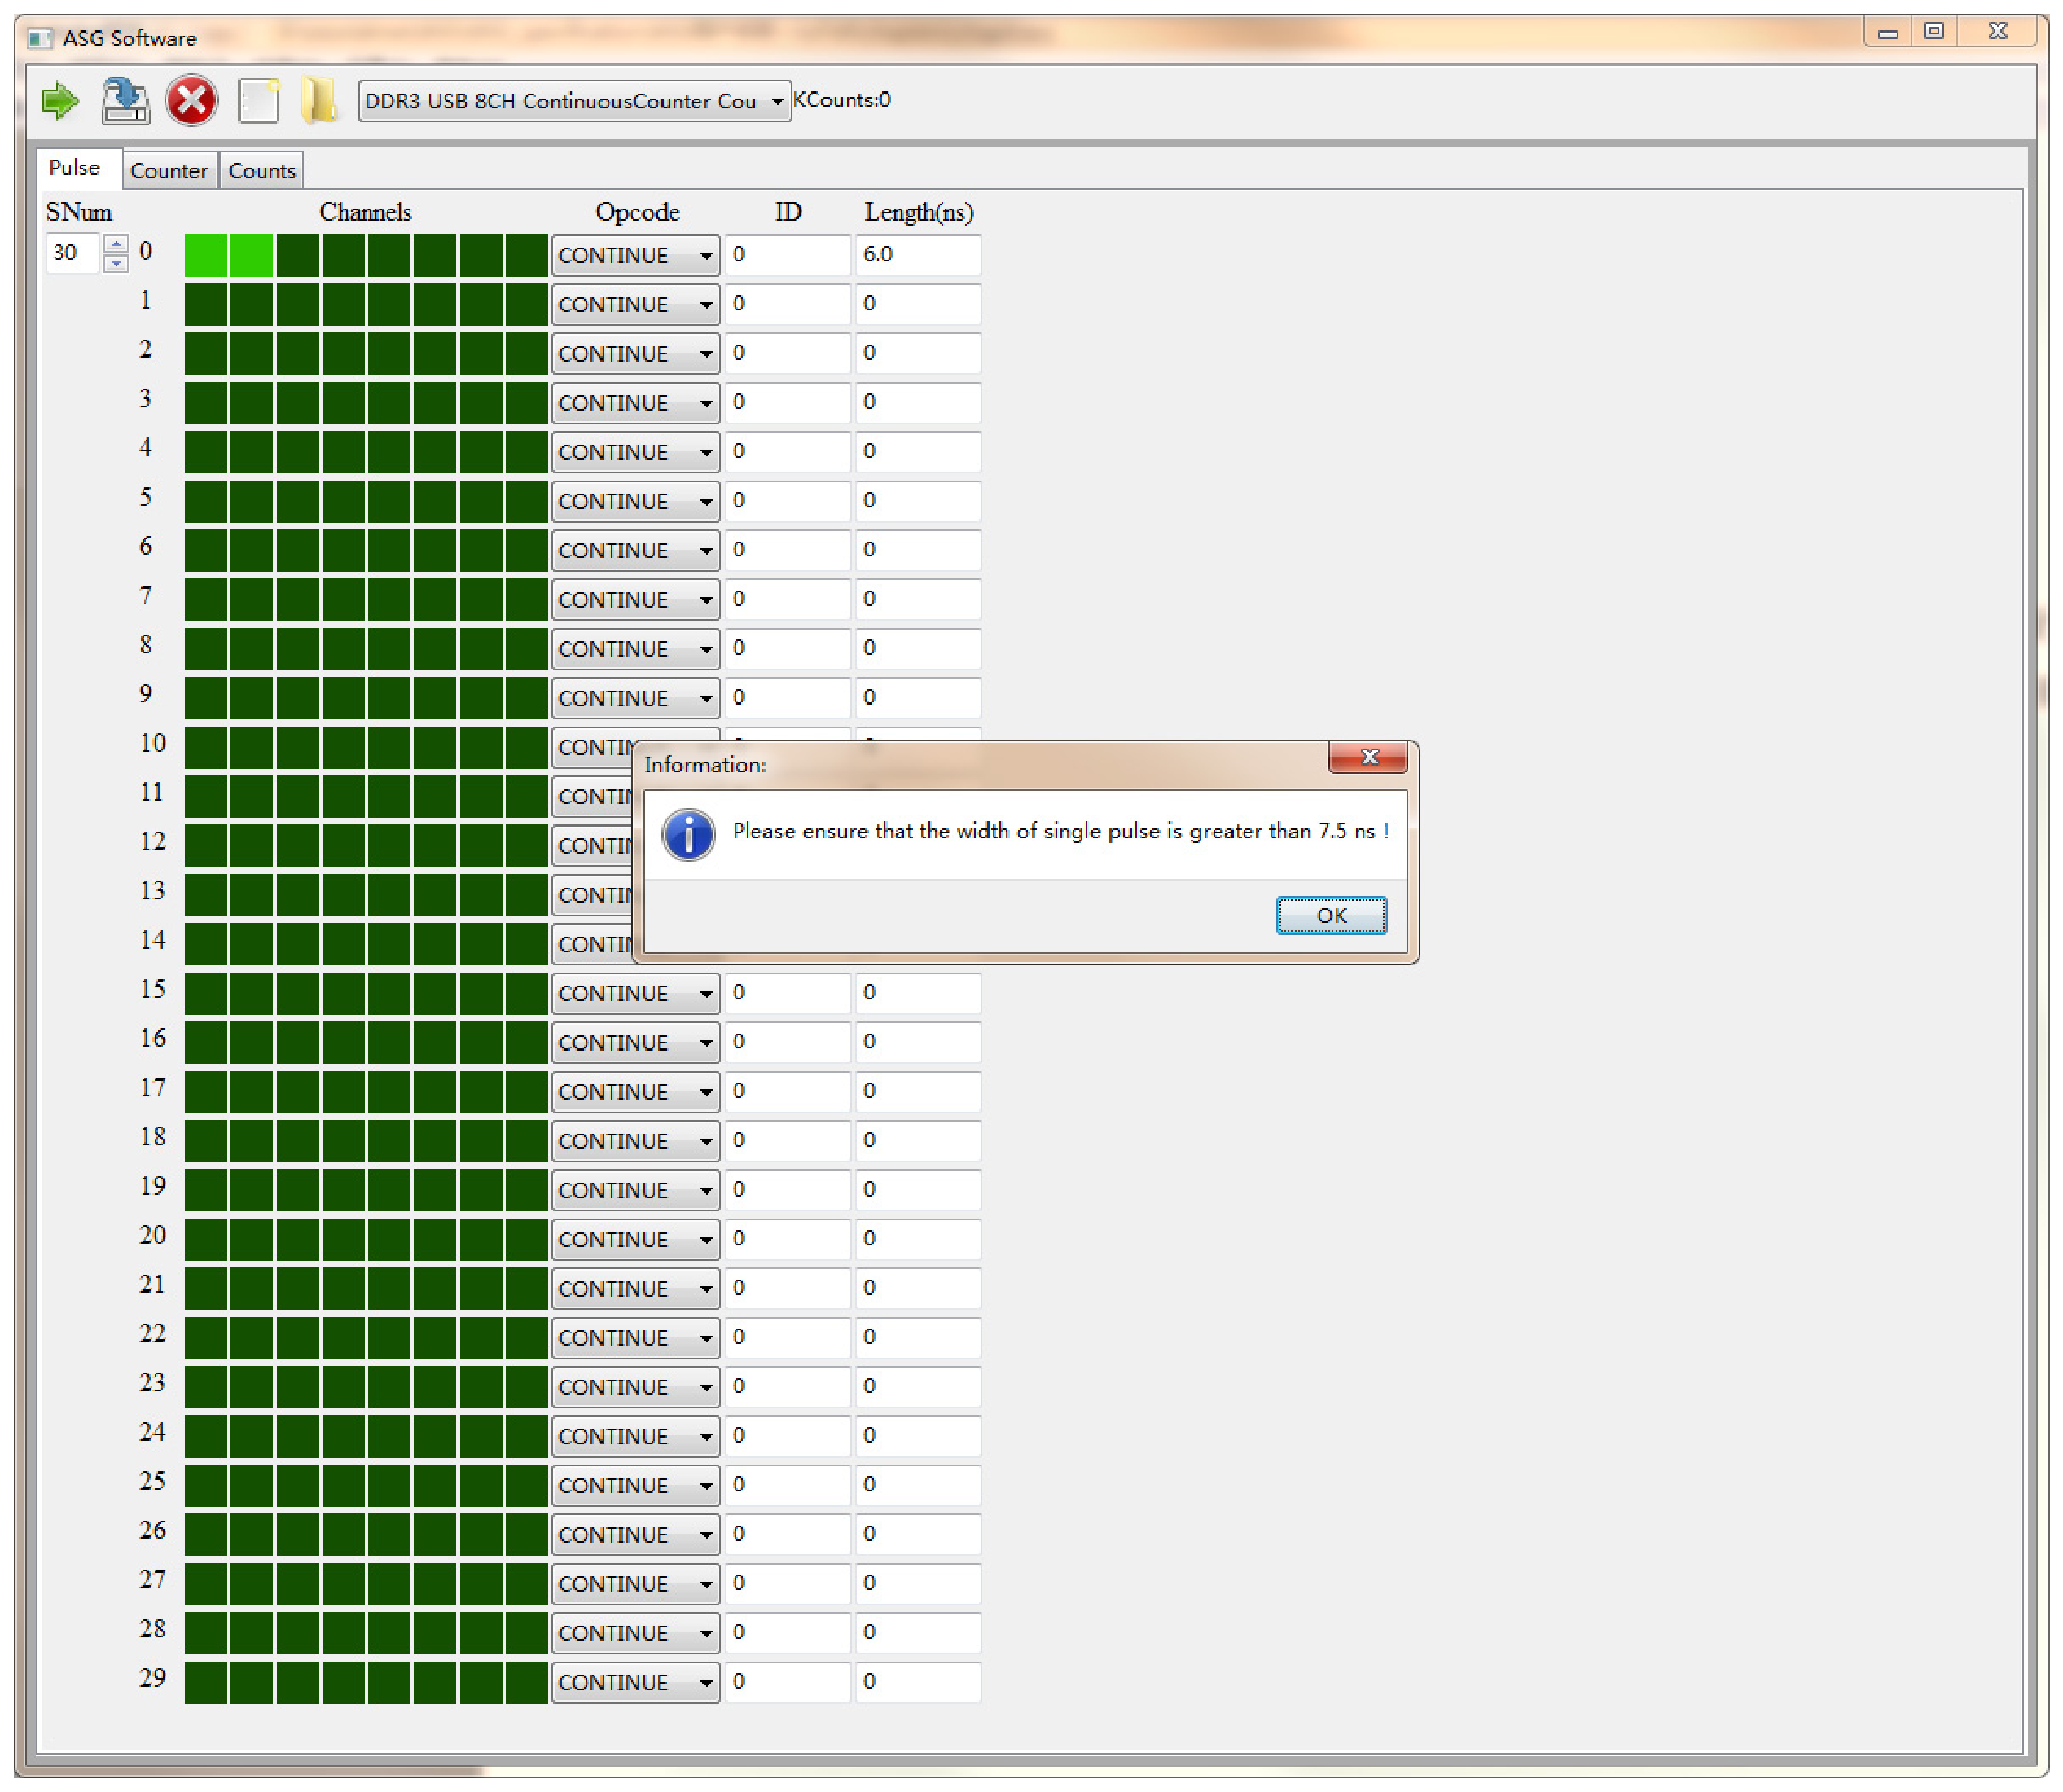
\includegraphics[width=11cm,height=9cm]{fig4_3}
%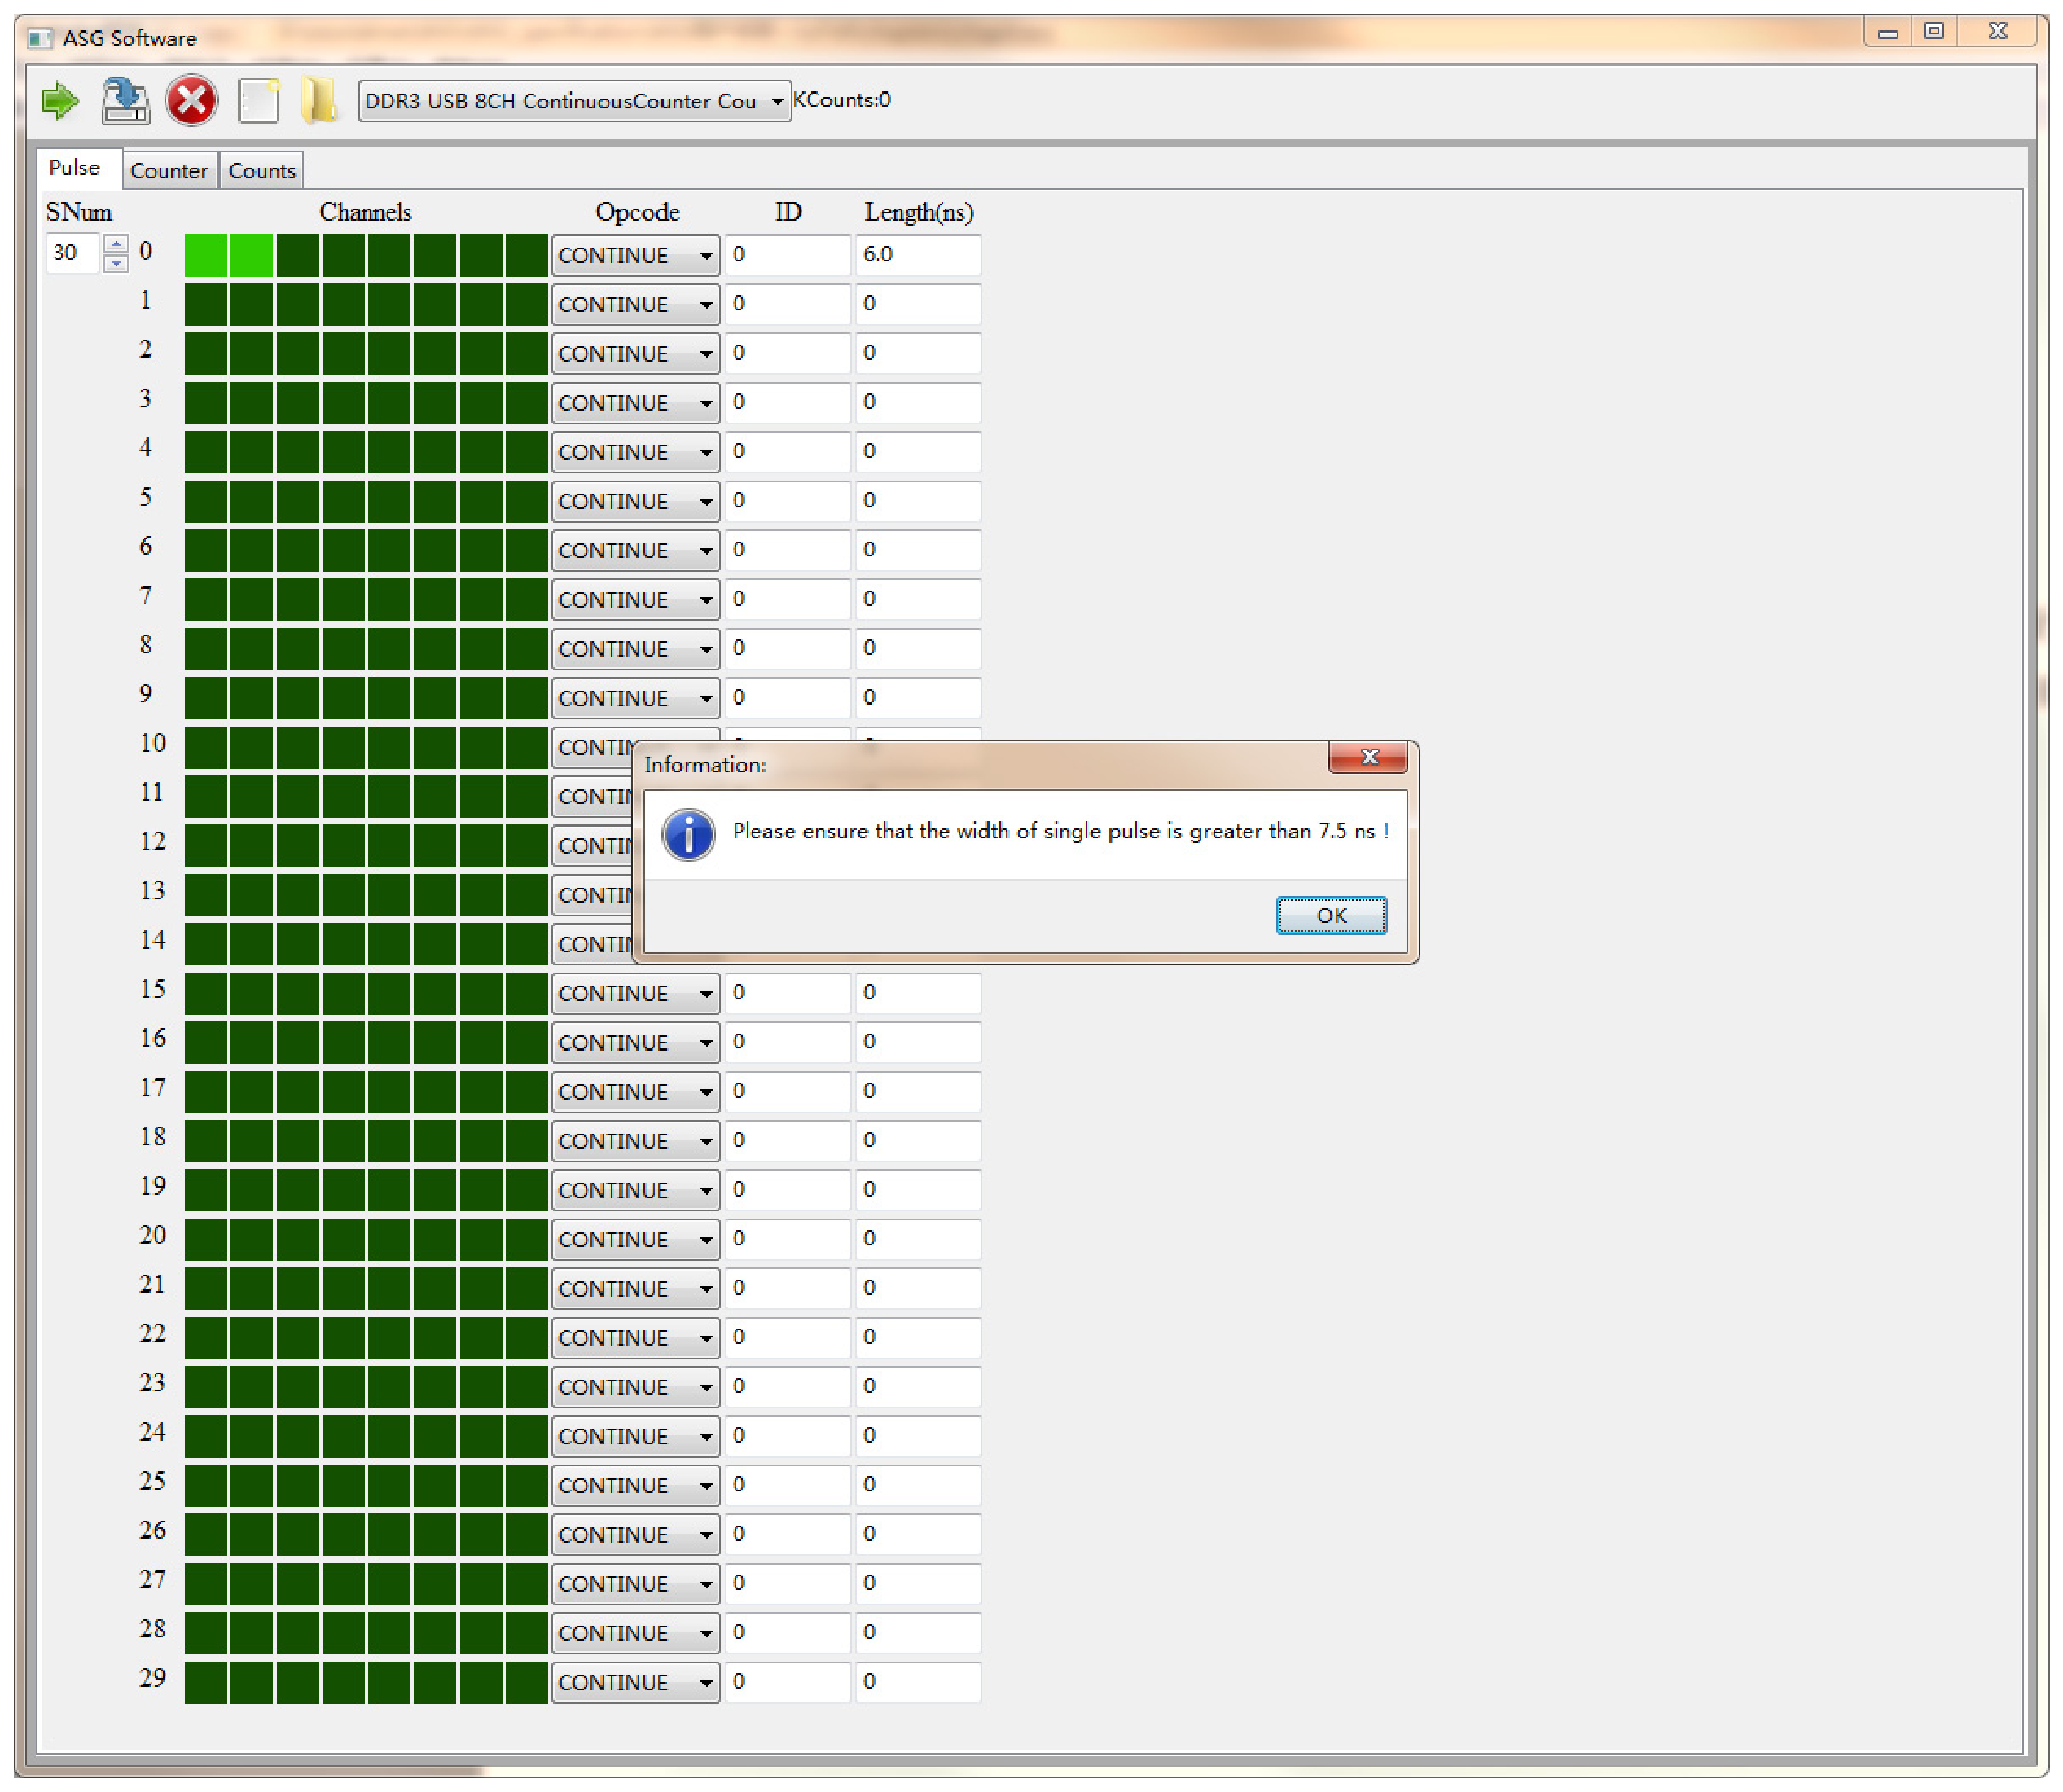
\includegraphics[height=9cm]{fig4_3}
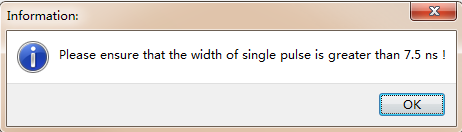
\includegraphics[height=3cm]{fig4_5_yh}
\caption{定义方波宽度小于7.5 ns提示}
\end{figure}

%\newpage
\vspace{0.4cm}
\noindent \textbf{(2)}.  如图4.6,当用户定义的方波序列中单个脉冲宽度大于2.6 s时,软件会弹出提示对话框。

\vspace{0.2cm}
\begin{figure}[ht]
\centering
%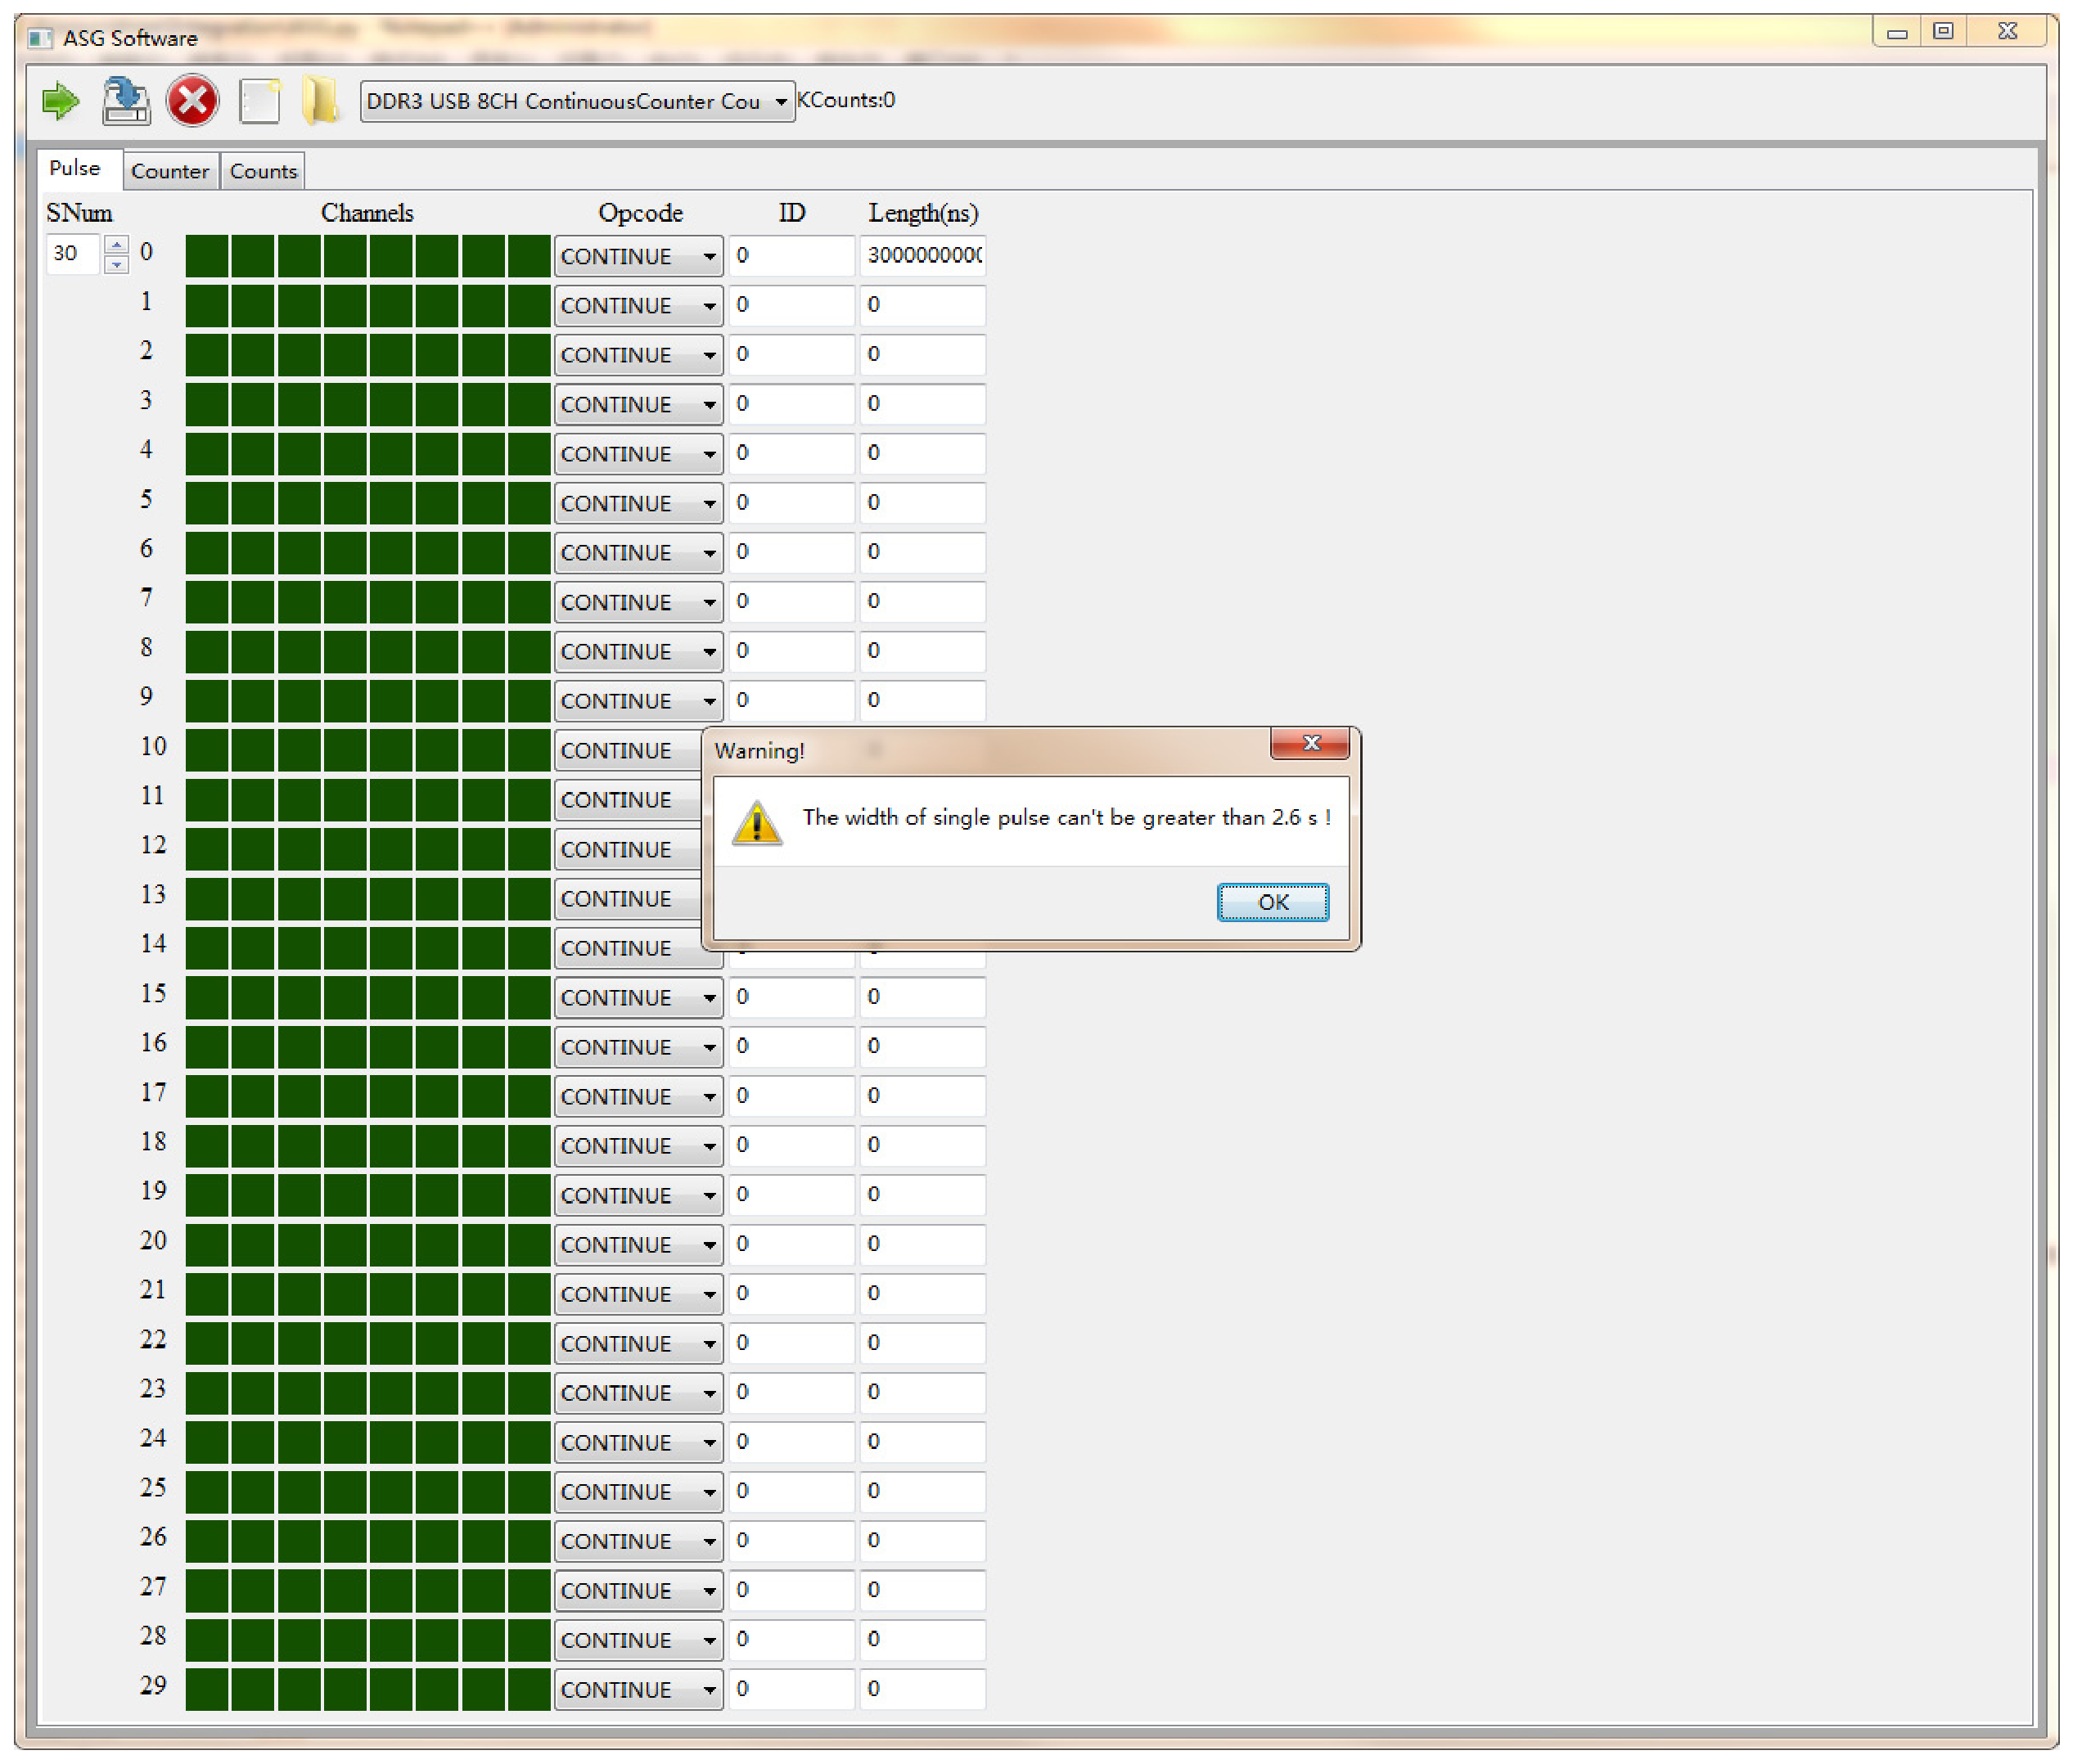
\includegraphics[width=11cm,height=9cm]{fig4_4}
%\includegraphics[height=9cm]{fig4_4yh}
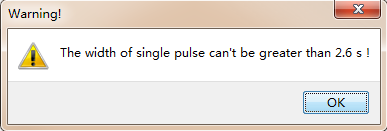
\includegraphics[height=3cm]{fig4_6_yh}
\caption{定义方波宽度大于2.6 s提示}
\end{figure}

\vspace{0.4cm}
\noindent \textbf{(3)}. 用户定义的每个方波序列的宽度必须是0.05 ns的整数倍。如图4.7,当用户定义的方波序列中存在单个方波脉冲宽度非0.05 ns整数倍时,软件会弹出提示对话框。

\vspace{0.2cm}
\begin{figure}[H]
\centering
%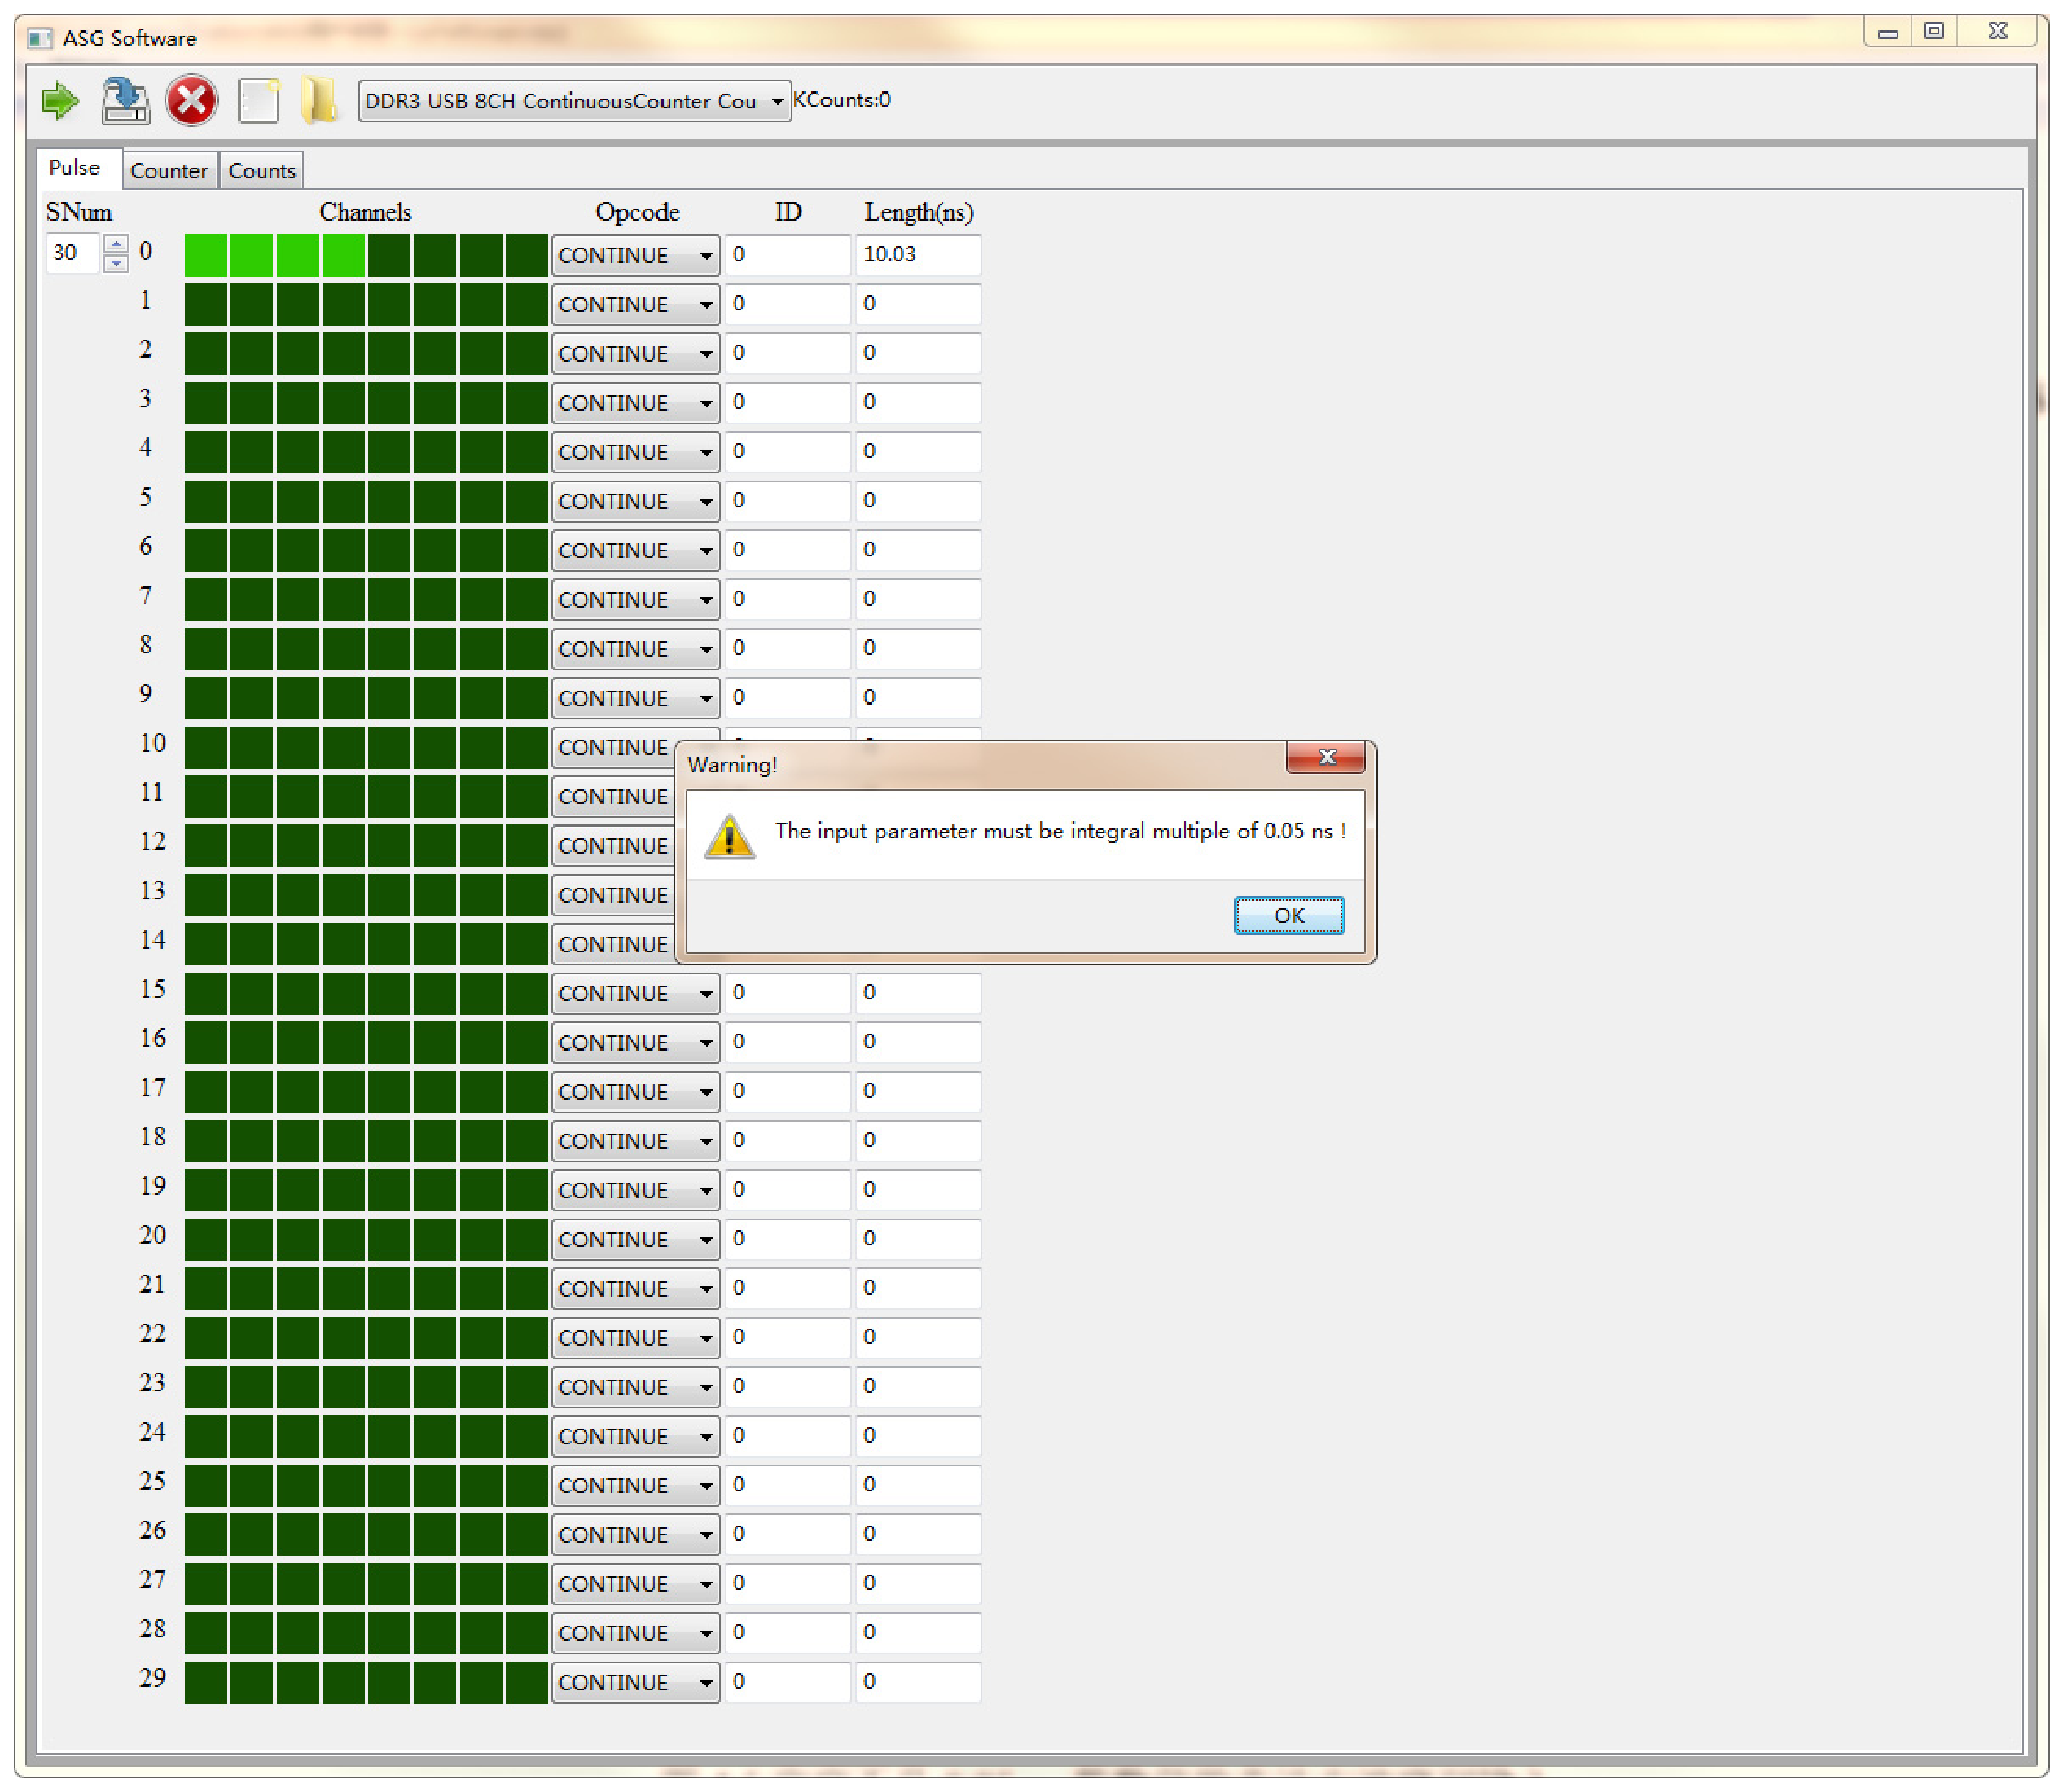
\includegraphics[width=11cm,height=9cm]{fig4_5}
%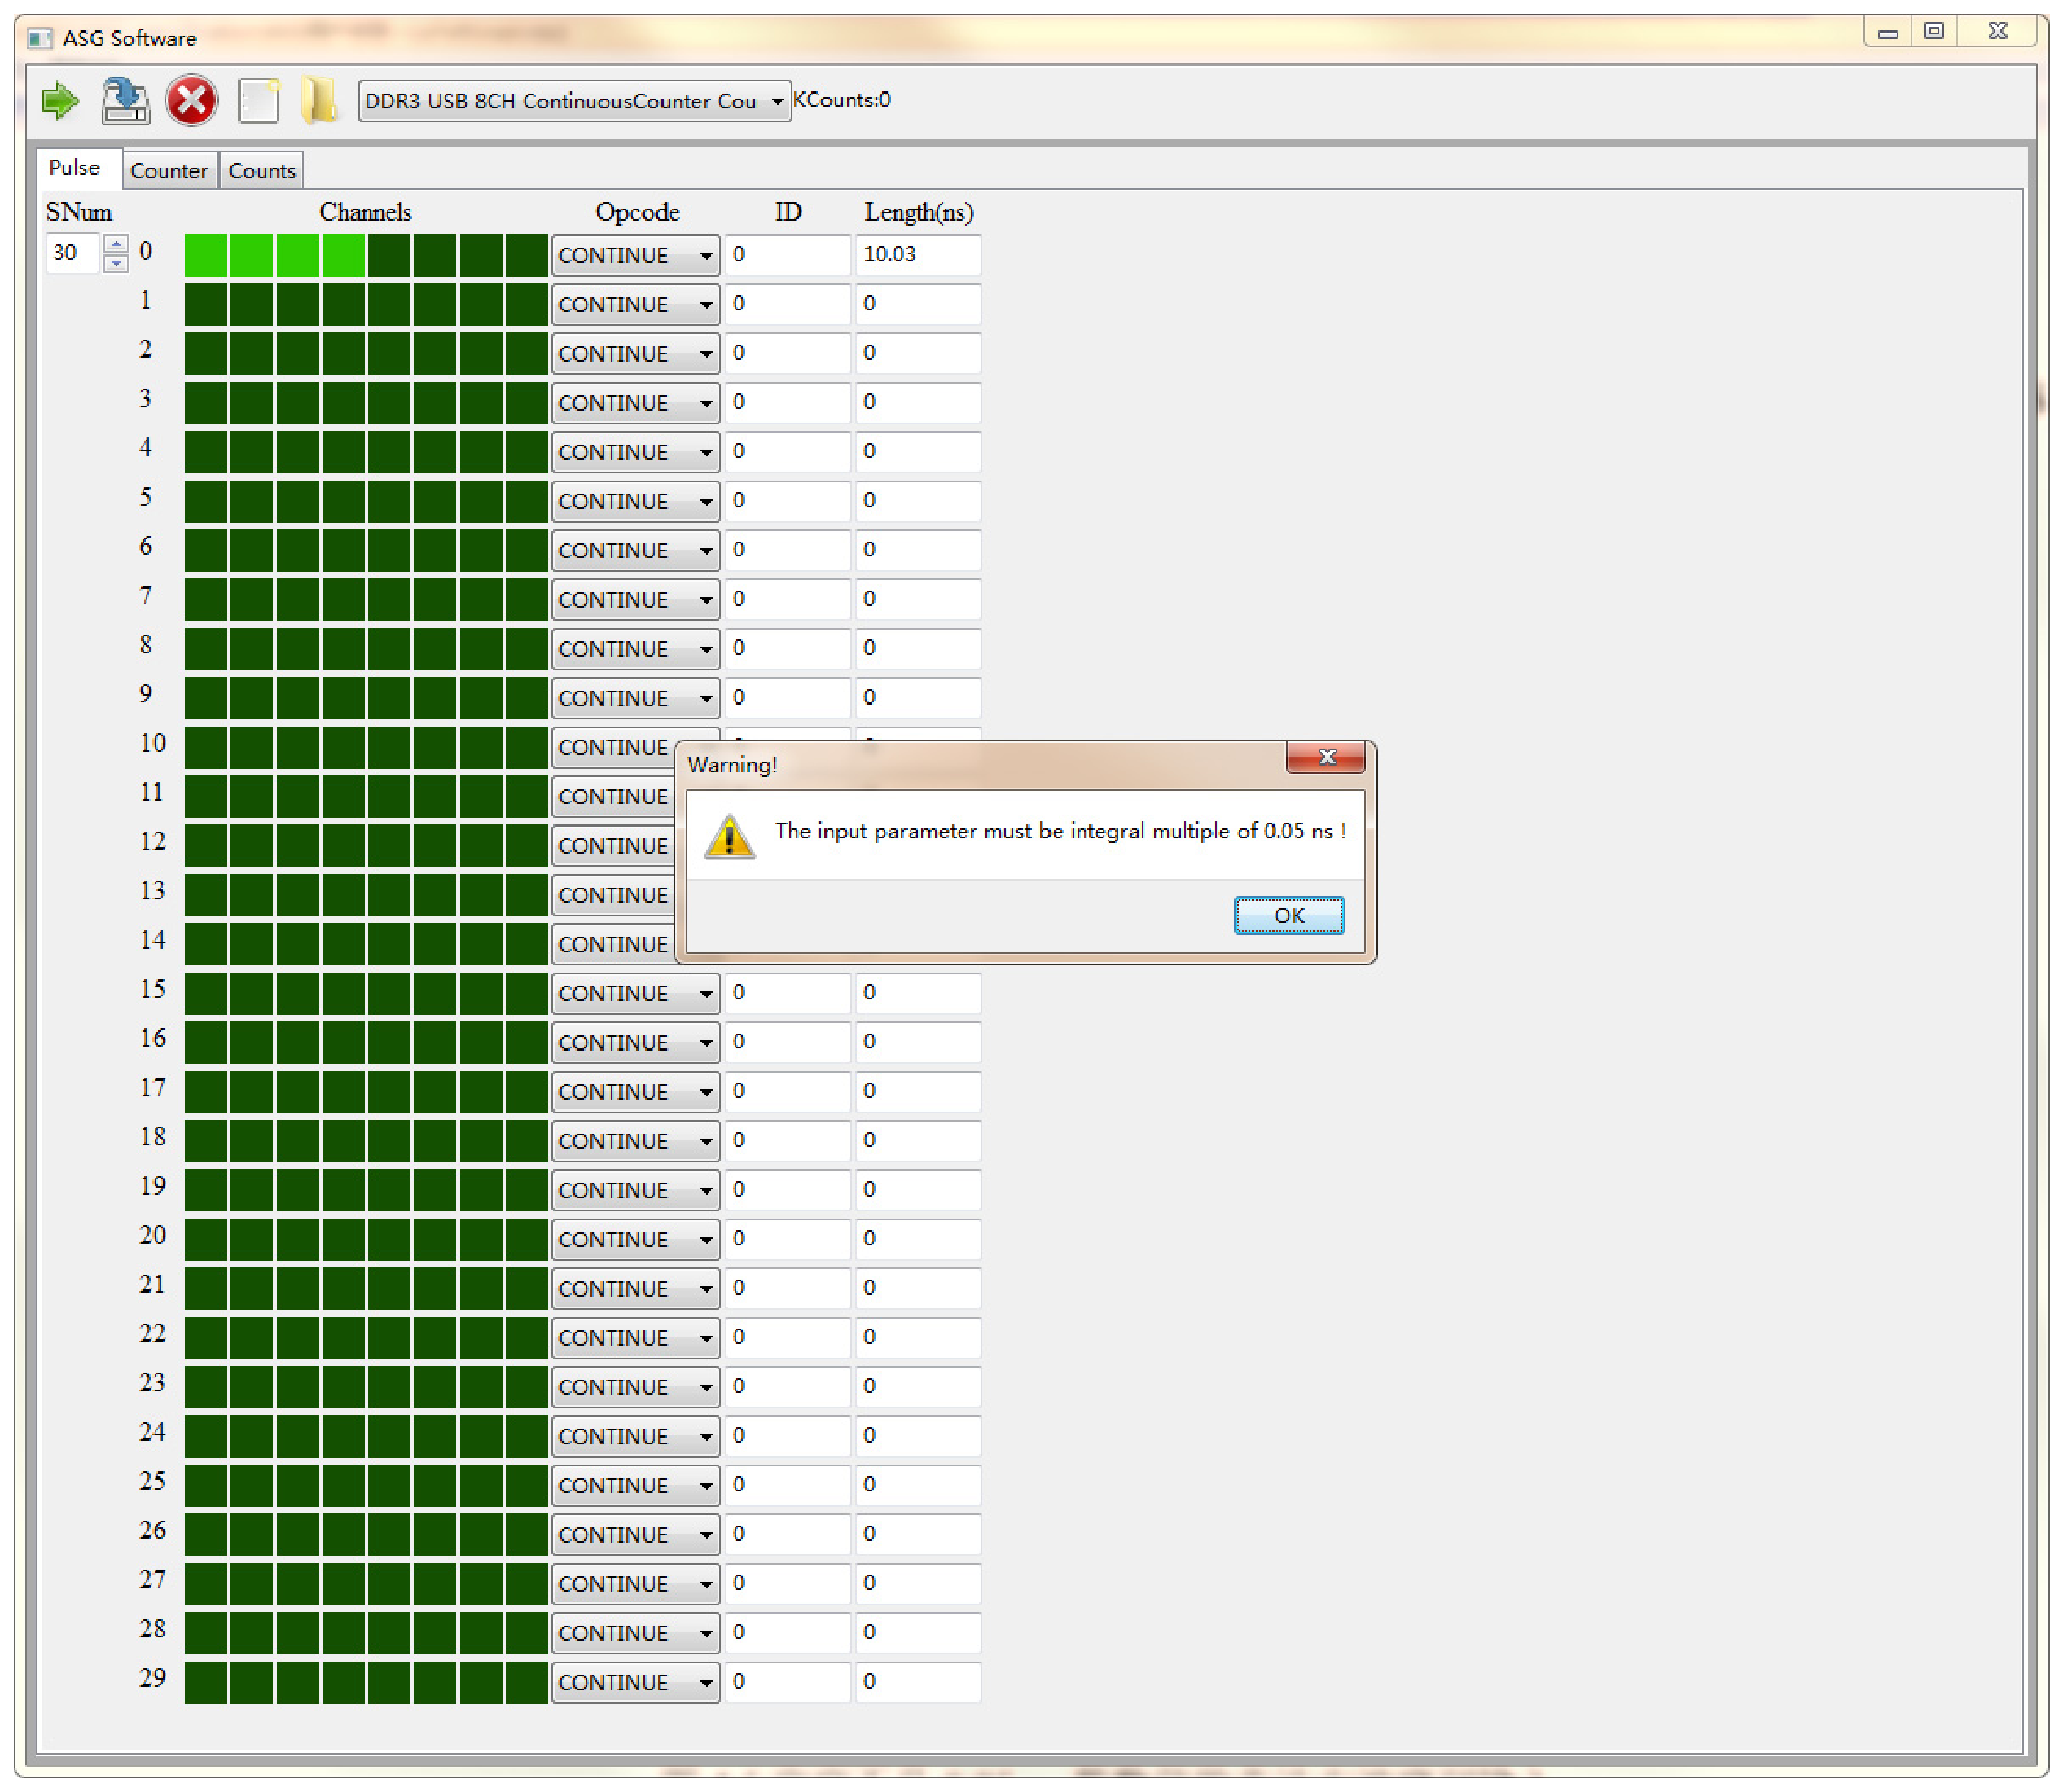
\includegraphics[height=9cm]{fig4_5}
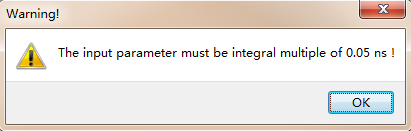
\includegraphics[height=3cm]{fig4_7_yh}
\caption{定义宽度不是0.05 ns整数倍提示}
\end{figure}

%\newpage
%\section{\heiti 开始播放方波序列}
%用户点击“Download”按钮
%
\includegraphics{download},可将自定义方波序列数据下载到硬件中。点击“Start”按钮{ }{ }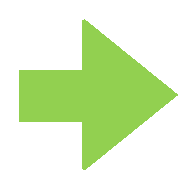
\includegraphics[height=0.7cm]{start},可使仪器各输出通道开始同步播放用户自定义的方波序列,在点击“Start” 按钮之前必须先将方波序列数据下载到硬件中。将输出通道用同轴线连接至示波器上可以看到仪器输出的方波波形。
%
%\section{\heiti 停止播放方波序列}
%当仪器正在播放方波序列时,可以通过点击“Stop”按钮{ }{ }
\includegraphics[height=0.7cm]{stop}使仪器停止播放方波序列。






\chapter{\heiti 调用接口程序}
\section{Python \heiti{接口程序}}
我司为用户提供了Python接口程序。用户可调用接口程序中的函数自己编程生成方波序列与计数通道使能序列,并将其下载到硬件中,然后控制仪器播放生成的方波序列以及读回计数结果。使用Python接口程序中的函数时可以参考我司为用户提供的“DDR3\_USB\_8chn\_ccounter\_dll.py”文件中的调用方式。现将用户所需的函数列出,并加以解释。注意在调用接口程序中的函数时,定义的单个方波序列高低电平时间必须在5 ns 至2.6 s 之间,且必须是0.05 ns的整数倍。定义的单个计数通道使能序列高低电平时间必须在5 ns至5000 s之间,且必须是5 ns的整数倍。
\vspace{0.4cm}

\noindent\fontsize{12pt}{\baselineskip}\textbf{\heiti{函数}PB\_type\_program(pulse)}

传入参数“pulse”是一个列表(list\_0),列表中的每个元素仍然是一个列表(list\_1),每个元素均形如[`01010101', 0, 0, 20.0]。list\_1中的第一个元素为一个字符串,字符串由8个‘0’或‘1’组成,从左往右依次代表8个输出通道,‘0’代表该通道输出低电平,‘1’代表该通道输出高电平。list\_1中的第二和第三个元素没有意义,为0即可。list\_1中的第四个元素代表该方波序列状态的持续时间,单位为纳秒。例如用户想要在OUT1通道输出一个高电平时间长度为60 ns低电平时间为40.05 ns的方波序列,则用户可以令pulse=[[`10000000',0,0,60], [`00000000',0,0,40.05]],然后调用PB\_type\_program(pulse)即可将该方波序列下载到硬件中。
\vspace{0.4cm}

\noindent\fontsize{12pt}{\baselineskip}\textbf{\heiti{函数}Counter\_program(pulse)}

传入参数“pulse”是一个列表(list\_2),列表中的每个元素仍然是一个列表(list\_3),每个元素均形如[`1',0,0,10.0]。list\_3中的第一个元素为‘0’或‘1’,‘0’代表计数通道使能序列为低电平,‘1’代表计数通道使能序列为高电平。list\_3中的第二和第三个元素没有意义,为0即可。list\_3中的第四个元素代表该计数通道使能序列状态的持续时间,单位为纳秒。例如用户想要生成一个高电平时间为20ns,低电平时间为15 ns 的计数通道使能序列,则用户可以令pulse=[[`1',0,0,20], [`0',0,0,15]],然后调用Counter\_program(pulse)即可将该计数通道使能序列下载到硬件中。

\newpage
\noindent\fontsize{12pt}{\baselineskip}\textbf{\heiti{函数}start()}

函数没有传入参数,在调用PB\_type\_program( )与Counter\_program( )后,再调用start( )即可向硬件发送指令使仪器开始播放方波序列以及开始计数。
\vspace{0.4cm}

\noindent\fontsize{12pt}{\baselineskip}\textbf{\heiti{函数}stop()}

此函数没有传入参数,用来向硬件发送指令,使仪器停止播放方波,并停止计数。在调用stop( )之后再次调用start( )可以重新使仪器播放方波序列并开始计数。
\vspace{0.4cm}

\noindent\fontsize{12pt}{\baselineskip}\textbf{\heiti{函数}get\_default\_count()}

此函数没有传入参数,可直接调用获得连续计数结果。
\vspace{0.4cm}

\noindent\fontsize{12pt}{\baselineskip}\textbf{\heiti{函数}get\_all\_count()}

此函数没有传入参数,可以直接调用获得计数结果。
\vspace{0.4cm}

\noindent\fontsize{12pt}{\baselineskip}\textbf{\heiti{完整调用过程举例}}

pulse = [[`10000000',0,0,60],[`00000000',0,0,40.05]]\qquad \#  定义方波序列

counter\_pulse = [[`1',0,0,60], [`0',0,0,15] ]\qquad        \#  定义计数通道使能序列

PB\_type\_program(pulse)\qquad            \#  下载方波序列

Counter\_program(counter\_pulse)\qquad     \#  下载方波序列

Start( )\qquad          \#  开始播放序列并开始计数

Continuous\_counter\_result = get\_default\_count()\qquad    \#  获得连续计数结果

Counter\_result = get\_all\_count()\qquad                  \#  获得计数结果

Stop( )\qquad     \#  停止播放序列并停止计数,仅在需要停止播放或计数时使用

\section{C\heiti 接口程序}
我司为用户提供了C接口程序。用户可调用接口程序中的函数自己编程生成方波序列与计数通道使能序列,并将其下载到硬件中然后控制仪器播放生成的方波序列以及读回计数结果。现将用户所需的函数列出,并作出解释。注意在调用接口程序中的函数时,定义的单个方波序列高低电平时间必须在5 ns至2.6 s之间,且必须是0.05 ns的整数倍。定义的单个计数通道使能序列高低电平时间必须在5 ns至5000 s之间,且必须是5 ns 的整数倍。

\newpage
\noindent\fontsize{12pt}{\baselineskip}\textbf{\heiti{函数}asg\_program\_all(char **flags,double *time\_length,unsigned long cmd\_num,\\unsigned char **buf,int *buf\_length)}
\begin{table}[H]
%\begin{table}[!htbp]
\Large
%\caption{}
\rowcolors{2}{gray!10}{gray!10}
\begin{tabular}{|m{7cm}<{\centering}|m{7cm}|}
%\begin{tabular}{p{0.5\textwidth}|p{0.5\textwidth}}
\rowcolor{gray!50}
\hline
传入参数 & \makebox[7cm][c]{参数描述} \\ \hline
char **flags & 参数“flags”是一个二维数组,每个元素均为形如“01011010”的字符串。字符串个数代表方波数据的个数,字符串中的‘0’或‘1’从左往右依次代表8个方波输出通道的的状态。‘0’ 代表低电平,‘1’ 代表高电平。\\ \hline
double *time\_length & 参数“time\_length”是一个double型一维数组。每个元素代表相应每个方波序列状态的时间长度,单位为纳秒。该数组长度必须与“flags”的数组长度相同。 \\\hline
unsigned long cmd\_num & 参数“cmd\_num”是一个正整数,表示方波序列数据的个数。 \\\hline
unsigned char **buf & 参数“buf”是一个二维空字符数组。即每个元素为一空字符串,字符串的个数为8,每个字符串的长为cmd\_num的10倍。 \\\hline
int *buf\_length & 参数“buf\_length”必须是\{0,0,0,0,0,0,0,0\}。 \\\hline
\end{tabular}
\end{table}

\newpage
\noindent\fontsize{12pt}{\baselineskip}\textbf{\heiti{函数}asg\_counter\_program\_all(char **flags, double *time\_length, unsigned long cmd\_num, unsigned char **buf,int *buf\_length)}
\begin{table}[H]
\Large
%\caption{}
\rowcolors{2}{gray!10}{gray!10}
\begin{tabular}{|m{7cm}<{\centering}|m{7cm}|}
\rowcolor{gray!50}
\hline
传入参数 & \makebox[7cm][c]{参数描述} \\ \hline
char **flags & 参数“flags”是一个二维数组,即每个元素均为形如“0”的字符串。字符串的个数代表方波的个数,字符串中的‘0’或‘1’代表计数通道使能序列的状态,‘0’代表低电平,‘1’代表高电平。\\ \hline
double *time\_length & 参数“time\_length”是一个double型数组。每个元素代表相应每个计数通道使能序列状态的时间长度,单位为纳秒。该数组长度必须与“flags”的数组长度相同。\\\hline
unsigned long cmd\_num & 参数“cmd\_num”是一个正整数,表示计数通道使能序列数据的个数。 \\\hline
unsigned char **buf & 参数“buf”是一个二维空字符数组。即每个元素为一空字符串,字符串的个数为1,每个字符串的长为cmd\_num的10倍。\\\hline
int *buf\_length & 参数“buf\_length”必须是\{0\}。 \\\hline
\end{tabular}
\end{table}
\vspace{0.4cm}

\noindent\fontsize{12pt}{\baselineskip}\textbf{\heiti{函数}asg\_start( )}

此函数没有传入参数,调用asg\_program\_all( )与asg\_counter\_program\_all( )后,再调用asg\_start( )即可向硬件发送指令使仪器开始播放方波序列以及开始计数。

\newpage
\noindent\fontsize{12pt}{\baselineskip}\textbf{\heiti{函数}asg\_stop( )}

 此函数没有传入参数,用来向硬件发送指令,使仪器停止播放方波,并停止计数。在调用asg\_stop( )之后再次调用asg\_start( )可以重新使仪器播放方波序列并开始计数。

\section{\heiti 两种接口程序比较}

现将Python接口程序与C接口程序中用户需要调用的函数做一对比,方便用户更好的理解调用接口程序的过程。
\begin{table}[H]
\Large
%\caption{}
%\rowcolors{2}{gray!10}{gray!10}
\begin{tabular}{|m{1.5cm}<{\centering}|m{5cm}<{\centering}|m{6.5cm}|}
\rowcolor{gray!50}
\hline
接口程序 & \makebox[6.6cm][l]{\qquad \qquad Python} & \makebox[6.0cm][c]{C}\\ \hline
\vspace{5cm}\multirow{4}{1in}{函数名} & PB\_type\_program(pulse)用来将方波数据下载到硬件中。& asg\_program\_all(char **flags, double *time\_length, unsigned long cmd\_num, unsigned char **buf, int *buf\_length)用来将方波数据下载到硬件中。\\\cline{2-3}
&Counter\_program(pulse)用来将计数通道使能序列数据下载到硬件中。& asg\_counter\_program\_all(char **flags, double *time\_length, unsigned long cmd\_num, unsigned char **buf, int *buf\_length)用来将计数通道使能序列数据下载到硬件中。\\\cline{2-3}
&start( )用来开始播放方波并开始计数。& asg\_start( )用来开始播放方波并开始计数。\\\cline{2-3}
&stop( )用来停止播放方波并停止计数。& asg\_stop( )用来停止播放方波并停止计数。\\
\hline
\end{tabular}
\end{table}
%\begin{figure}
%\centering
%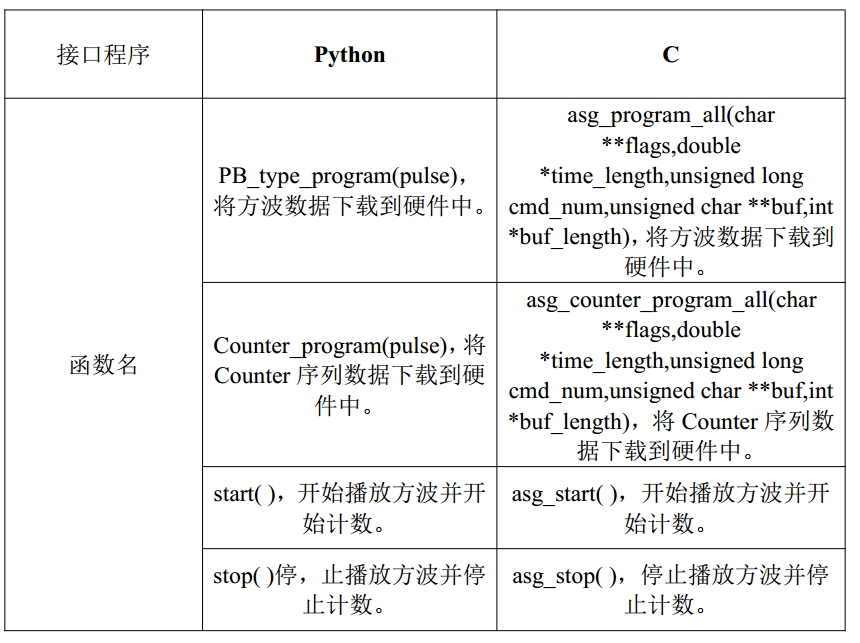
\includegraphics[width=16cm]{last_table}
%\end{figure}

\chapter{\heiti In MAC OSX}
\section{\heiti{Startup}}

\noindent Download the SDK from 
\\{http://www.cypress.com/documentation/software-and-drivers/ez-usb-fx3-software-development-kit}
\\ \\
Uncompress the SDK file:FX3\_SDK\_MacOS\_v1.3.3.tar.gz
\\ \\ 
And uncompress the file:cyusb\_mac\_1.0.tar.gz
\\ \\
Open the `docs' folder, and refer to `cyusb\_mac\_user\_guide.pdf'. You can start from the Section 2.1.

\begin{enumerate}
\item Install the library `libusb'.
\item Enter the `lib' folder and run `make' command in the terminal. Then copy the `*.dylib' file to the \/usr\/local\/lib.
\item Copy the configs\/cyusb.conf to \/etc folder.
\item Uncompress the file we provided and enter the directory which just be generated and run `.\/cybulk\_writer 512' command in the terminal. A demo signal is generated by the device and you could see it on the oscilloscope.
\item If fail, you should use the `cybulk\_writer.c' we provided to replace the same file in the  `examples' directory and run `make' command in the terminal. You will get many executable files. Then run `.\/cybulk\_writer 512' command again.
\end{enumerate}

\section{\heiti{API Introduction}}

We also provide API written in Python. The filename is `macosx\_pulse\_api.py'. Before you running the script, you must install python interpreter and package `numpy'. The Python script use the program `cybulk\_writer' to download data to the device. So they must exist in the same folder.
\\
\indent For the example to use the Python script, please refer to the functions `delay\_chain\_test' and `random\_pulse\_test' in the script. You can also run the script in the terminal. If all is configured well, the device will output signal.
\\
\indent We provide 3 API functions for the user: PB\_type\_program, start and stop. For more information, please refer to the comment in the function.
\\

Parameter for the function `PB\_type\_program':

\vspace{0.2cm}
\begin{table}[H]
%\begin{table}[!htbp]
\normalsize
%\caption{}
%\rowcolors{2}{gray!10}{gray!10}
\begin{tabular}{|m{6.5cm}<{\centering}|m{7cm}<{\centering}|}
%\begin{tabular}{p{0.5\textwidth}|p{0.5\textwidth}}
% \rowcolor{blue!50}
\hline Parameter Type & List[List[String, Float]...]
\\ 
\hline Example 1 & [['00001111', 10.0], ['11110000', 10.05]] 
\\ 
\hline Example 2 & [['10000000', 10.0], ['11000000', 0.05], ['01000000', 15.0]] \\\hline
\end{tabular}
\end{table}

\begin{figure}[ht]
\centering
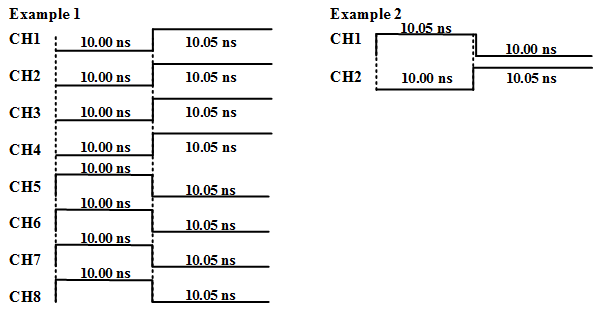
\includegraphics[height=6cm]{pulse_example_mac}
\caption{Example waveform}
\label{pulse_example_mac}
\end{figure}

\indent API calling example:

\begin{figure}[ht]
\centering
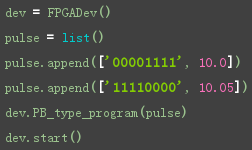
\includegraphics[height=4cm]{program_example_mac}
\caption{Program example}
\label{program_example_mac}
\end{figure}


\section{\heiti{Understand the Data Structure of the Pulse Sequence}}
\indent We use 10 bytes (80-bit) to describe a pulse with high level and low level. Each 80-bit data includes 32-bit high level time data, 32-bit low level time data, 5-bit leading edge delay data, 5-bit trailing edge delay data, and 6 reserved bits. 

\begin{table}[H]
\centering
\normalsize
\begin{tabular}{|m{3.5cm}|m{3.5cm}|m{0.5cm}|m{1cm}|m{0.5cm}|m{1cm}|}
% \rowcolor{blue!50}
\hline 32-bit & 32-bit & \qquad & 5-bit & \qquad & 5-bit \\\hline
\end{tabular}
\end{table}

\indent The least bit of the 32-bit data represents 0.625 ns for high level time or low level time. And the 5-bit data adjust the edge of the pulse with 50 ps resolution.
\indent A complicated pulse sequence consists of many 10 bytes elements. By utilizing the different storage space of DDR3, it can define arbitrary pulse sequence freely.
\chapter{\heiti 故障处理}
下面列举了ASG-GT50-C 在使用过程中可能出现的故障及排查方法。当您遇到这些故障时,请按照相应的步骤进行处理,如不能处理,请与我司联系。

\section{\heiti 计算机无法识别仪器}
在已经安装过USB驱动程序的计算机上连接仪器,然而在计算机的设备管理器中发现无法识别设备,请重新插拔USB连接线并检查USB连接线是否有损伤。确认USB连接线完好,并多次重新插拔后仍无法识别设备,请及时与我司联系。

\section{\heiti 设置正确但无方波信号输出}
\noindent {\textcircled{\normalsize{\textbf{1}}}}. 检查SMA线缆是否与相应的通道输出端口(OUT1 - OUT8)紧固连接。

\noindent {\textcircled{\normalsize{\textbf{2}}}}. 检查SMA线缆是否有内部损伤。

\noindent {\textcircled{\normalsize{\textbf{3}}}}. 检查SMA线缆是否与测试仪器紧固连接。

\noindent {\textcircled{\normalsize{\textbf{4}}}}. 以上三条均检查无误后,若仍无方波信号输出,请及时与我司联系。


\section{\heiti 无计数结果读回}
\noindent {\textcircled{\normalsize{\textbf{1}}}}. 检查定义的计数通道使能序列是否满足要求。

\noindent {\textcircled{\normalsize{\textbf{2}}}}. 检查外部输入信号是否正常,且输入信号频率在最大计数率(50 MHz)内。

\noindent {\textcircled{\normalsize{\textbf{3}}}}. 如果定义的计数通道使能序列满足需求,且外部输入信号正常,但仍无计数

\hspace{-0.5em}结果读回,请与我司联系。
%\begin{enumerate}
%\item 检查定义的Counter序列是否满足要求。
%\item 检查外部输入信号是否正常,并且输入信号频率在最大计数率(50 MHz)内。
%\item 如果定义的Counter序列满足需求,且外部输入信号正常,却仍无计数结果读\\
%\end{enumerate}

\chapter{\heiti Application Notices}
\section{\heiti Hardware part}
\noindent {\textcircled{\normalsize{\textbf{1}}}}. The working environment temperature of ASG-GT50-C must be within -10 $^{\circ}$C to +50 $^{\circ}$C .
%\noindent {\textcircled{\normalsize{\textbf{1}}}}. 任意序列发生器的外界工作环境温度必须在-10 $^{\circ}$C 至 +50 $^{\circ}$C以内。

\noindent {\textcircled{\normalsize{\textbf{2}}}}. Be careful when handling the instrument, and do not place heavy objects on top of the chassis.
%\noindent {\textcircled{\normalsize{\textbf{2}}}}. 搬运仪器时请轻拿轻放,切勿将重物放置在机箱上。

%\section{\heiti 软件注意事项}
%\noindent {\textcircled{\normalsize{\textbf{1}}}}. Windows安装的Python解释器必须为Python 2.7版本以上,但不能是Python3

%\hspace{-0.3em}版本以上。

%\noindent {\textcircled{\normalsize{\textbf{2}}}}. 建议用户安装32位的Python解释器。若用户已安装了64位的Python解释
%
%\hspace{-0.3em}器,我司会为用户提供需要更新的DLL文件。

%\noindent {\textcircled{\normalsize{\textbf{2}}}}. 为用户提供的“ASG\_install”文件夹请勿放在系统盘(C盘)中。
\section{\heiti Others}
\noindent {\textcircled{\normalsize{\textbf{1}}}}. If you suspect damage occurs to the instrument, have it inspected by our company authorized personnel before further operation. Any maintenance, adjustment or replacement especially to circuits or accessories must be performed by our company authorized personnel, or we don't assume any responsibility.

%\hspace{-0.2cm}何由未经我司允许的维护、 调整或零件更换而造成损失, 我司概不承担任何

%\hspace{-0.2cm}责任。

%\noindent {\textcircled{\normalsize{\textbf{1}}}}.如果您怀疑本产品出现故障, 请立即联络我司授权的维修人员进行检测。任

%\hspace{-0.2cm}何由未经我司允许的维护、 调整或零件更换而造成损失, 我司概不承担任何

%\hspace{-0.2cm}责任。


\newpage
\qquad

\newpage
\qquad
\thispagestyle{empty}

\newpage
%\begin{titlepage}
\newgeometry{left=0cm,right=0cm,top=0cm,bottom=0cm}
\begin{center}
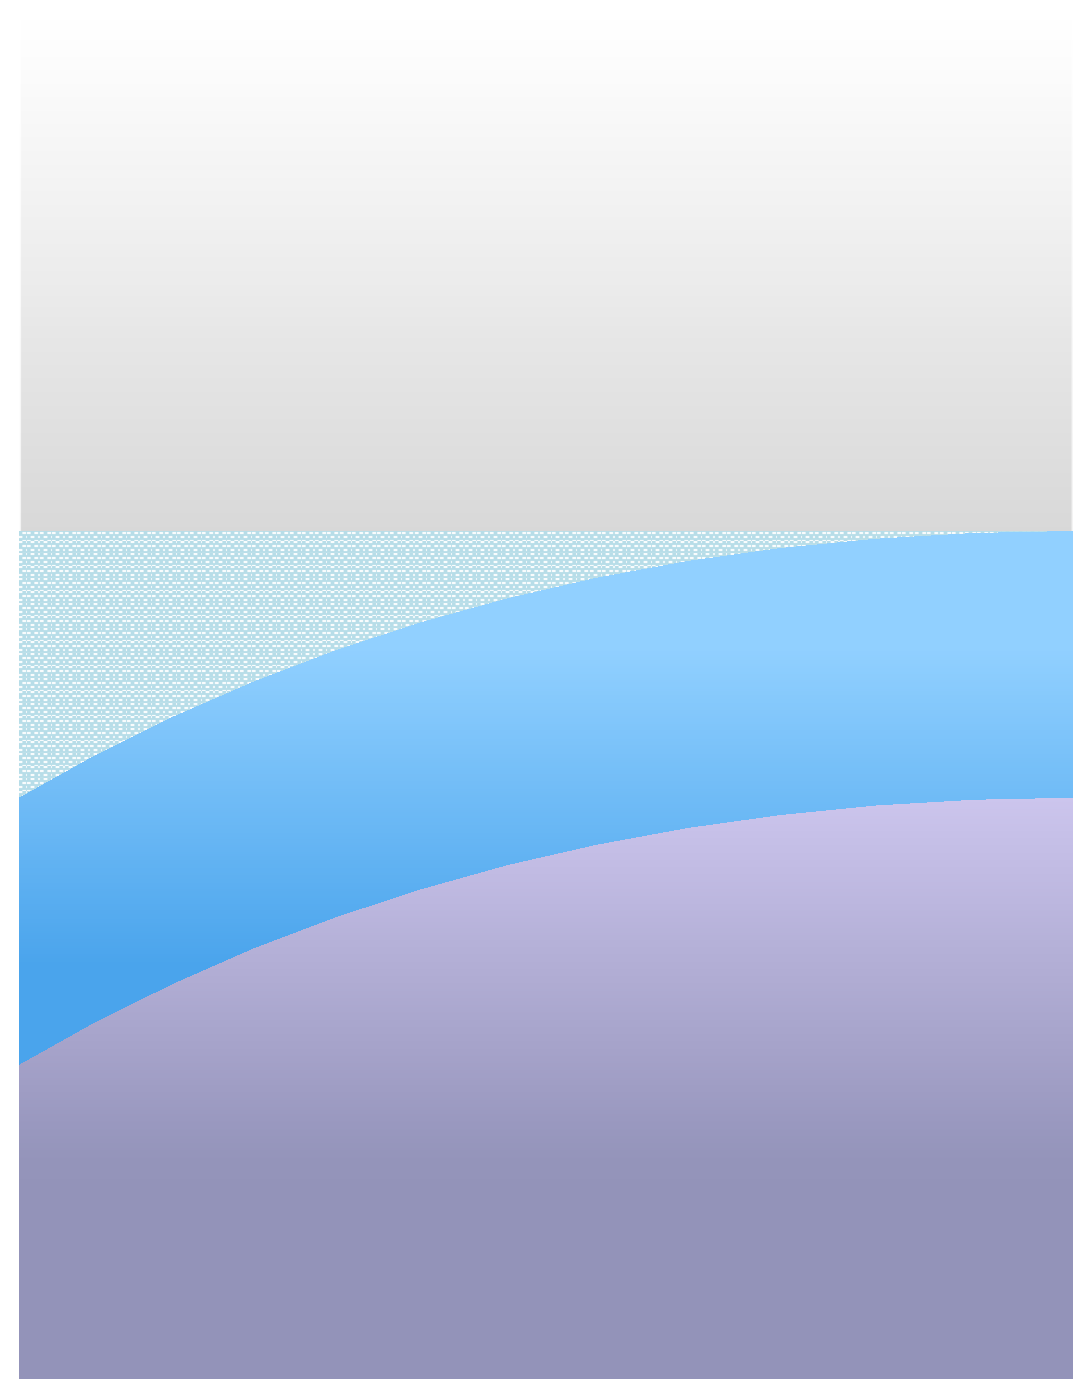
\includegraphics[width=20.99cm,height=29.6cm]{titlepage2}
\end{center}
%\end{titlepage}



\end{document}


